%%%%%%%%%%%%%%%%%%%%%%%%%%%%%%%%%%%%%%%%%
% Programming/Coding Assignment
% LaTeX Template
%
% This template has been downloaded from:
% http://www.latextemplates.com
%
% Original author:
% Ted Pavlic (http://www.tedpavlic.com)
%
% Note:
% The \lipsum[#] commands throughout this template generate dummy text
% to fill the template out. These commands should all be removed when 
% writing assignment content.
%
% This template uses a Perl script as an example snippet of code, most other
% languages are also usable. Configure them in the "CODE INCLUSION 
% CONFIGURATION" section.
%
%%%%%%%%%%%%%%%%%%%%%%%%%%%%%%%%%%%%%%%%%

%----------------------------------------------------------------------------------------
%	PACKAGES AND OTHER DOCUMENT CONFIGURATIONS
%----------------------------------------------------------------------------------------

\documentclass{article}

\usepackage{fancyhdr} % Required for custom headers
\usepackage{lastpage} % Required to determine the last page for the footer
\usepackage{extramarks} % Required for headers and footers
\usepackage[usenames,dvipsnames]{color} % Required for custom colors
\usepackage{graphicx} % Required to insert images
\usepackage{listings} % Required for insertion of code
\usepackage{courier} % Required for the courier font
\usepackage{lipsum} % Used for inserting dummy 'Lorem ipsum' text into the template
\usepackage[utf8]{inputenc} % Required for inputting international characters
\usepackage[T1]{fontenc} % Output font encoding for international characters
\usepackage{pdfpages}

% Margins
\topmargin=-0.45in
\evensidemargin=0in
\oddsidemargin=0in
\textwidth=6.5in
\textheight=9.0in
\headsep=0.25in

\linespread{1.1} % Line spacing

% Set up the header and footer
\pagestyle{fancy}
\lhead{\hmwkTitle} % Top left header
\rhead{\hmwkAuthorName} % Top right header
%\chead{\hmwkClass\ (\hmwkClassInstructor\ \hmwkClassTime): \hmwkTitle} % Top center head
%\rhead{\firstxmark} % Top right header
\lfoot{\lastxmark} % Bottom left footer
\cfoot{} % Bottom center footer
\rfoot{Strana\ \thepage\ - \protect\pageref{LastPage}} % Bottom right footer
\renewcommand\headrulewidth{0.4pt} % Size of the header rule
\renewcommand\footrulewidth{0.4pt} % Size of the footer rule

\setlength\parindent{0pt} % Removes all indentation from paragraphs

%----------------------------------------------------------------------------------------
%	CODE INCLUSION CONFIGURATION
%----------------------------------------------------------------------------------------

\definecolor{MyDarkGreen}{rgb}{0.0,0.4,0.0} % This is the color used for comments
\lstloadlanguages{C++} % Load C++ syntax for listings
\lstset{language=C++, % Use c++ in this example
        frame=single, % Single frame around code
        basicstyle=\small\ttfamily, % Use small true type font
        keywordstyle=[1]\color{Blue}\bf, % c++ functions bold and blue
        keywordstyle=[2]\color{Purple}, % c++ function arguments purple
        keywordstyle=[3]\color{Blue}\underbar, % Custom functions underlined and blue
        identifierstyle=, % Nothing special about identifiers                                         
        commentstyle=\usefont{T1}{pcr}{m}{sl}\color{MyDarkGreen}\small, % Comments small dark green courier font
        stringstyle=\color{Purple}, % Strings are purple
        showstringspaces=false, % Don't put marks in string spaces
        tabsize=5, % 5 spaces per tab
        %
        % Put standard c++ functions not included in the default language here
        morekeywords={rand},
        %
        % Put c++ function parameters here
        morekeywords=[2]{on, off, interp},
        %
        % Put user defined functions here
        morekeywords=[3]{test},
       	%
        morecomment=[l][\color{Blue}]{...}, % Line continuation (...) like blue comment
        numbers=left, % Line numbers on left
        firstnumber=1, % Line numbers start with line 1
        numberstyle=\tiny\color{Blue}, % Line numbers are blue and small
        stepnumber=5 % Line numbers go in steps of 5
}

% Creates a new command to include a perl script, the first parameter is the filename of the script (without .pl), the second parameter is the caption
\newcommand{\perlscript}[2]{
\begin{itemize}
\item[]\lstinputlisting[caption=#2,label=#1]{#1.pl}
\end{itemize}
}

%----------------------------------------------------------------------------------------
%	DOCUMENT STRUCTURE COMMANDS
%	Skip this unless you know what you're doing
%----------------------------------------------------------------------------------------

% Header and footer for when a page split occurs within a problem environment
\newcommand{\enterProblemHeader}[1]{
\nobreak\extramarks{#1}{#1 pokračování na další straně\ldots}\nobreak
\nobreak\extramarks{#1 (pokračování)}{#1 pokračování na další straně\ldots}\nobreak
}

% Header and footer for when a page split occurs between problem environments
\newcommand{\exitProblemHeader}[1]{
\nobreak\extramarks{#1 (pokračování)}{#1 pokračování na další straně\ldots}\nobreak
\nobreak\extramarks{#1}{}\nobreak
}

%----------------------------------------------------------------------------------------
%	NAME AND CLASS SECTION
%----------------------------------------------------------------------------------------

\newcommand{\hmwkTitle}{Konvexní obálky a jejich konstrukce} % Assignment title
\newcommand{\hmwkDueDate}{Datum odevzdání: 26.11.2017} % Due date
\newcommand{\hmwkClass}{155ADKG} % Course/class
%\newcommand{\hmwkClassTime}{10:30am} % Class/lecture time
%\newcommand{\hmwkClassInstructor}{Jones} % Teacher/lecturer
\newcommand{\hmwkAuthorName}{Petra~Millarová, ~Oleksiy~Maybrodskyy} % Your name

%----------------------------------------------------------------------------------------
%	TITLE PAGE
%----------------------------------------------------------------------------------------

\title{
\vspace{2in}
\textmd{\textbf{\hmwkClass:\ \hmwkTitle}}\\
\normalsize\vspace{0.1in}\large{\hmwkDueDate}\\
%\vspace{0.1in}\large{\textit{\hmwkClassInstructor\ \hmwkClassTime}}
\vspace{3in}
}

\author{\textbf{\hmwkAuthorName}}
\date{} % Insert date here if you want it to appear below your name

%----------------------------------------------------------------------------------------

\begin{document}

\maketitle

%----------------------------------------------------------------------------------------
%	TABLE OF CONTENTS
%----------------------------------------------------------------------------------------

%\setcounter{tocdepth}{1} % Uncomment this line if you don't want subsections listed in the ToC

\newpage
\tableofcontents
\newpage

%----------------------------------------------------------------------------------------
%	PROBLEM 1
%----------------------------------------------------------------------------------------

% To have just one problem per page, simply put a \clearpage after each problem

\section{Zadání}
\indent Následuje kopie oficiálního zadání úlohy. Autoři z nepovinných bodů zadání úspěšně implementovali algoritmus pro ošetření singulárního případu u Jarvis Scan: existence kolineárních bodů v data, rozpracovana kontrukce konvexní obálky metodou Graham Scan.
\begin{figure}[htbp]
    \centering
        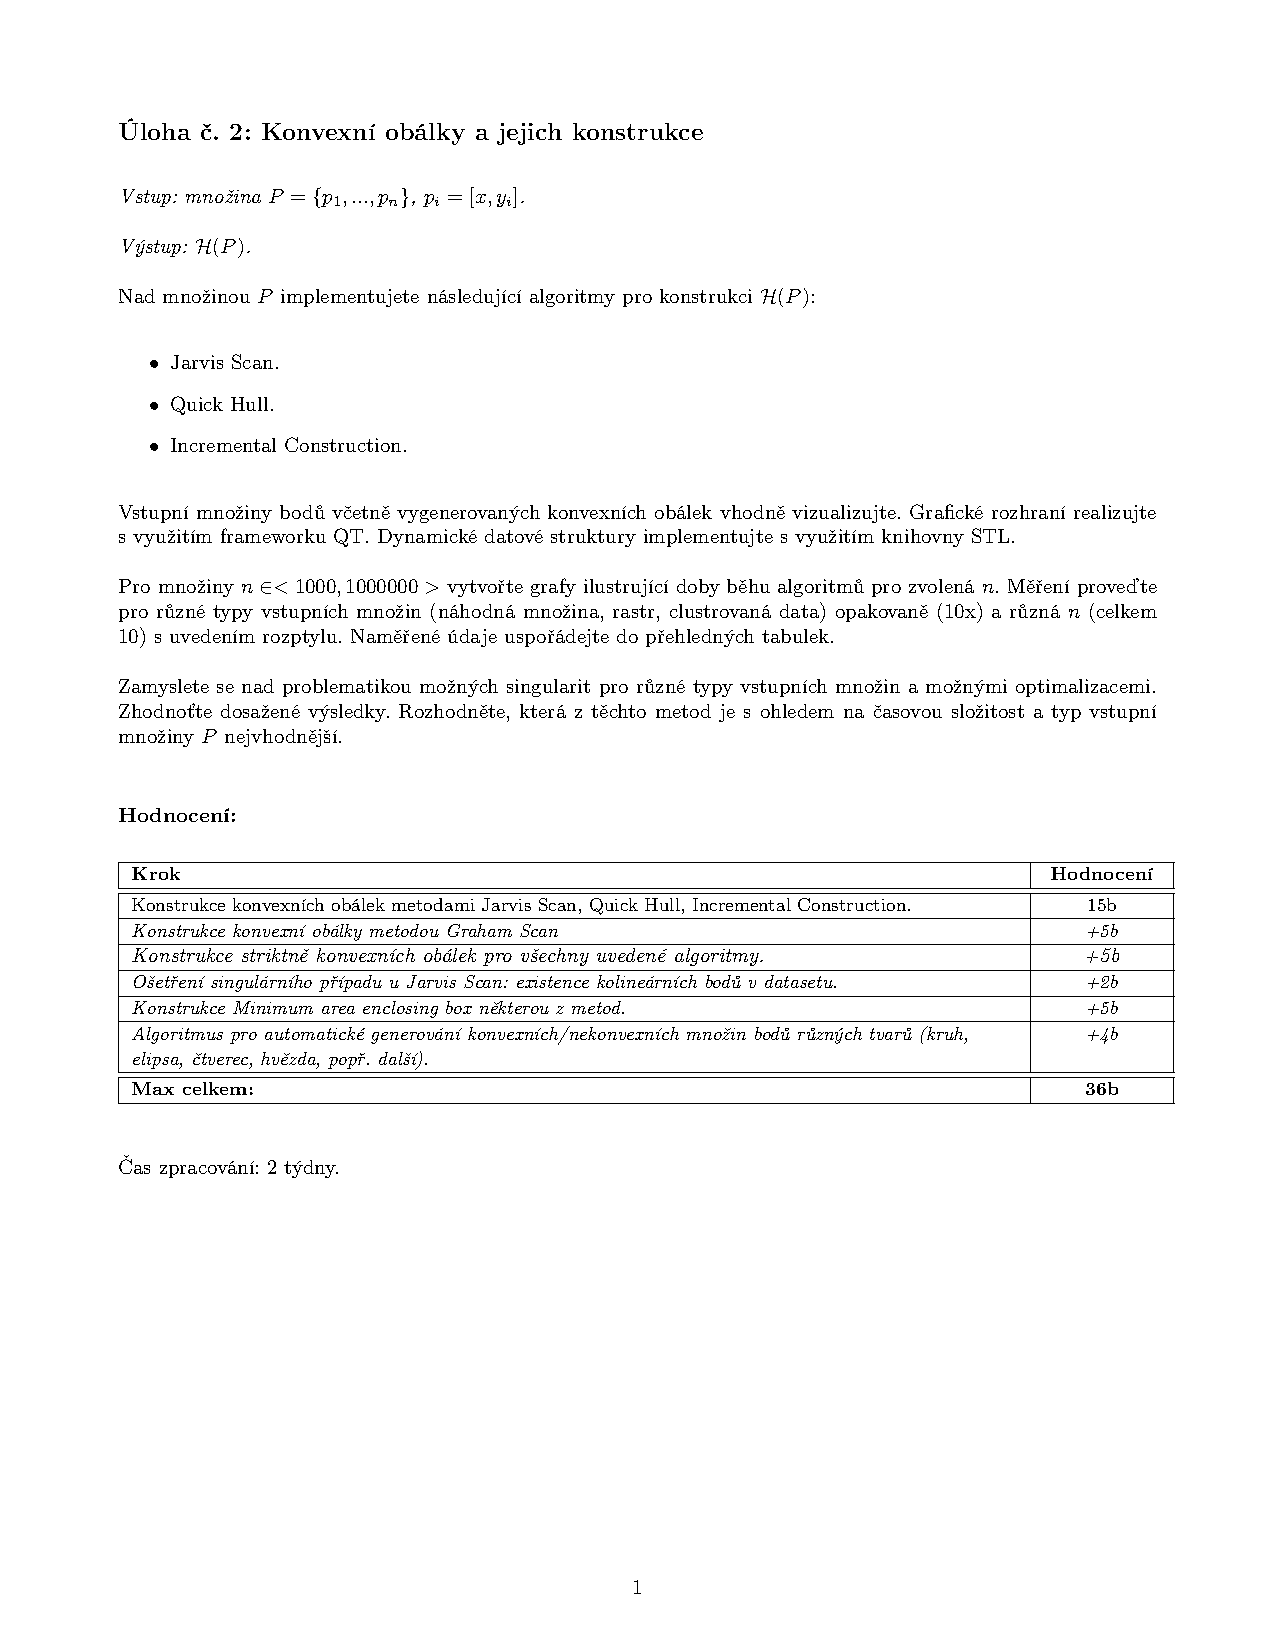
\includegraphics[clip, trim=0cm 7cm 0cm 0cm, width=1.00\textwidth]{zadani.pdf}
\end{figure}
\clearpage
\section{Popis a rozbor problému} %+vzorce
\indent 
Tato úloha se věnuje řešení praktického problému konvexní obálky pro náhodné množiny bodů, pravidelné množiny bodů. Jako implementaci si lze zjednodušeně představit vytvarování digitální mapy. 
\\
\\
\clearpage
\section{Popisy algoritmů} %formálním jazykem
V dané úloze jsou použity následující algoritmy, avšak existují i další možnosti, jak polohu bodu určit.
\subsection{Jarvis Scan}
 Jedna se o dost pomalý algoritmus oprotí ostatním algoritmům zabývájicím se obdobním problémy. Algoritmus funguje na principu gip wrapping, česky balení dárku.\\
\bigskip
Nechť v kartezské soustavě souřadnic existuje množina bodů. Setřiděním souřadnic dle osy  \textit{\textbf {Y}}, je možné najít počáteční bod \textit{\textbf {q}} (dále jen pivot), který je dan obrázek bodu s nejmenší hodnotou na ose \textit{\textbf {Y}}. Dále předpokladáme, že v množině uvedených bodů neexistují 3 kolineární body. Pak je možné aplikovat níže uvedený algoritmus:\\
\bigskip
\begin{enumerate}
\item Nalezení pivota $q$ = min($y_i$),
\item Vklad $q$ do množiny $H$.
\item $p_j$ = q, $p_i$ = $p_{j-1}$.
\item Načítání bodu $p_{j-1}$
\item  $p_i$ $\ne$ q:
\item Cyklus pro body $p_{j-1}$, $p_j$:
\item Dokud $p_i$ je takové, že $\theta$ = min($\theta_i$);
\item Vklad do množiny  $H$.
\end{enumerate}
\clearpage
\newpage
\subsection{Quick Hull} 

Algoritmus typu QuikSort. Konvexní obálka tvořena z horní a dolní částí.\\
Horní část obsahuje body nad spojnicí bodů a dolní část je pod spojnicí $q_1$ a $q_3$.\\
Řešení pro káždou konvexní obálku se provádí zvlašť a následně se sloučuje. Hledáme nejvzdalenější bod pro káždou konvexní obálku ležící vpravo od této strany. Nově vzníklý bod se stává bodem obálky. Nově vzníklá strana se rozděluje na dvě nové strany, princip rozděluj a panuj.\\
\bigskip
\subsection{Incremental Construcion}

Inkrementální algoritmus je velmi rychlý algoritmus pro výpočet konvexní obalky. Princip se základa na postupným testováním bodů, respektive jejich předaváním do konvexní obalky, jejiž tvar je modefikovan.\\
\bigskip
\clearpage
\newpage
\section{Vstupní data}
Aplikace má 2 mody.  První mod znázorňuje výsledky výpočtu obrázem situace.Mezi vstupními daty patří jediná hodnota, a to koknretně uživatelem zadaná hodnota požadovaného počtu bodů. Generovát lze na základě randomného, respektve náhodného rozložení, nebo na základě gridu, respektive pravidelné síti bodů. V rámci třetí možností je třeba ještě uvést náhodného generování shluku bodů.
\bigskip
Druhý mod, respektive Graph mode vytváří graf, který znázorňuje generování v konkretních metodach v intervalu od 1000 do 1000000 a úkláda výsledky grafů do formatu .PDF.
\bigskip
\clearpage
\newpage
\section{Výstupní data}
Výstup je vizualizací řešeného problému v grafickém okně. Taky v grafickém okně je slovně napsana rychlost výpočtu algoritmu.\\ 
\bigskip 
Praktickým výstupem je graf znázorňující rychlot výpočtu algoritmu v podobě vykreslování grafu. Uživátel si sam zvolí umistění. Víc další kapitoly\\ 
\bigskip 
\clearpage
\section{Ukázky aplikace} %printscreen
\bigskip
\begin{figure}[htbp]
\centering
        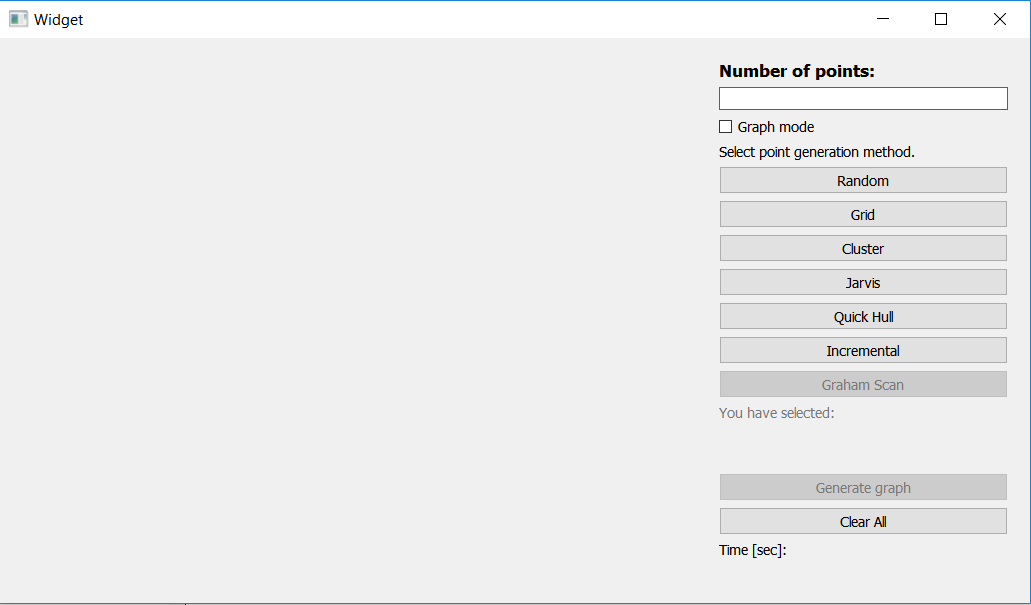
\includegraphics[clip, trim=0cm 0cm 0cm 0cm, width=1\textwidth]{obrazek1.png}
        \caption{Aplikace po spuštění}
\end{figure}
\begin{figure}[htbp]
\centering
        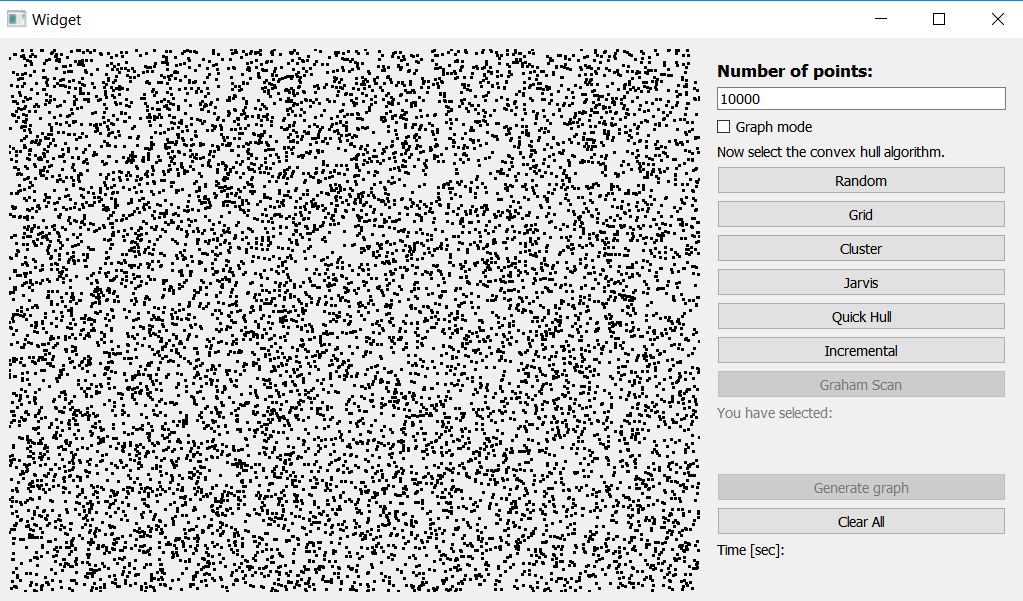
\includegraphics[clip, trim=0cm 0cm 0cm 0cm, width=1\textwidth]{obrazek2.png}
        \caption{Aplikace po spuštění RANDOM}
\end{figure}
\begin{figure}[htbp]
\centering
        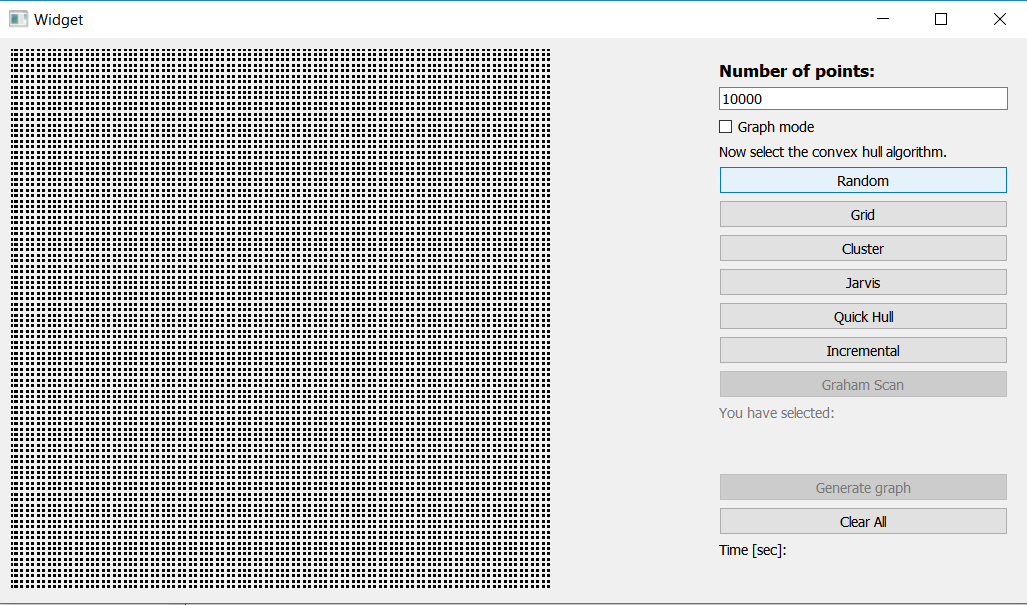
\includegraphics[clip, trim=0cm 0cm 0cm 0cm, width=1\textwidth]{obrazek3.png}
        \caption{Aplikace po spuštění GRID}
\end{figure}
\begin{figure}[htbp]
\centering
        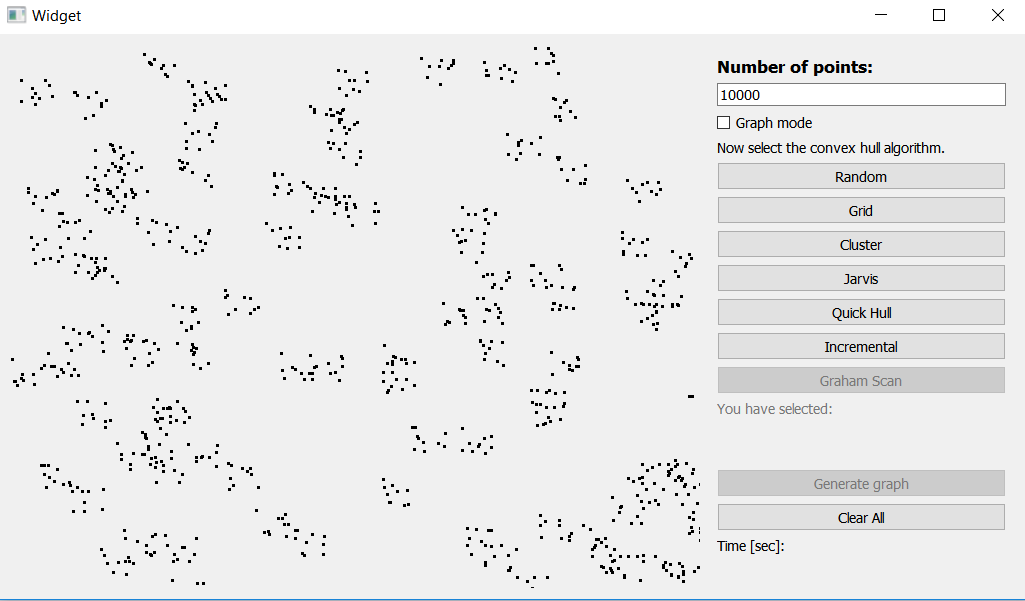
\includegraphics[clip, trim=0cm 0cm 0cm 0cm, width=1\textwidth]{obrazek4.png}
        \caption{Aplikace po spuštění Cluster}
\end{figure}
\clearpage
\newpage
\subsection{RANDOM}
\textit{\textbf {Jarvis Scan}}
\\
\begin{figure}[htbp]
\centering
        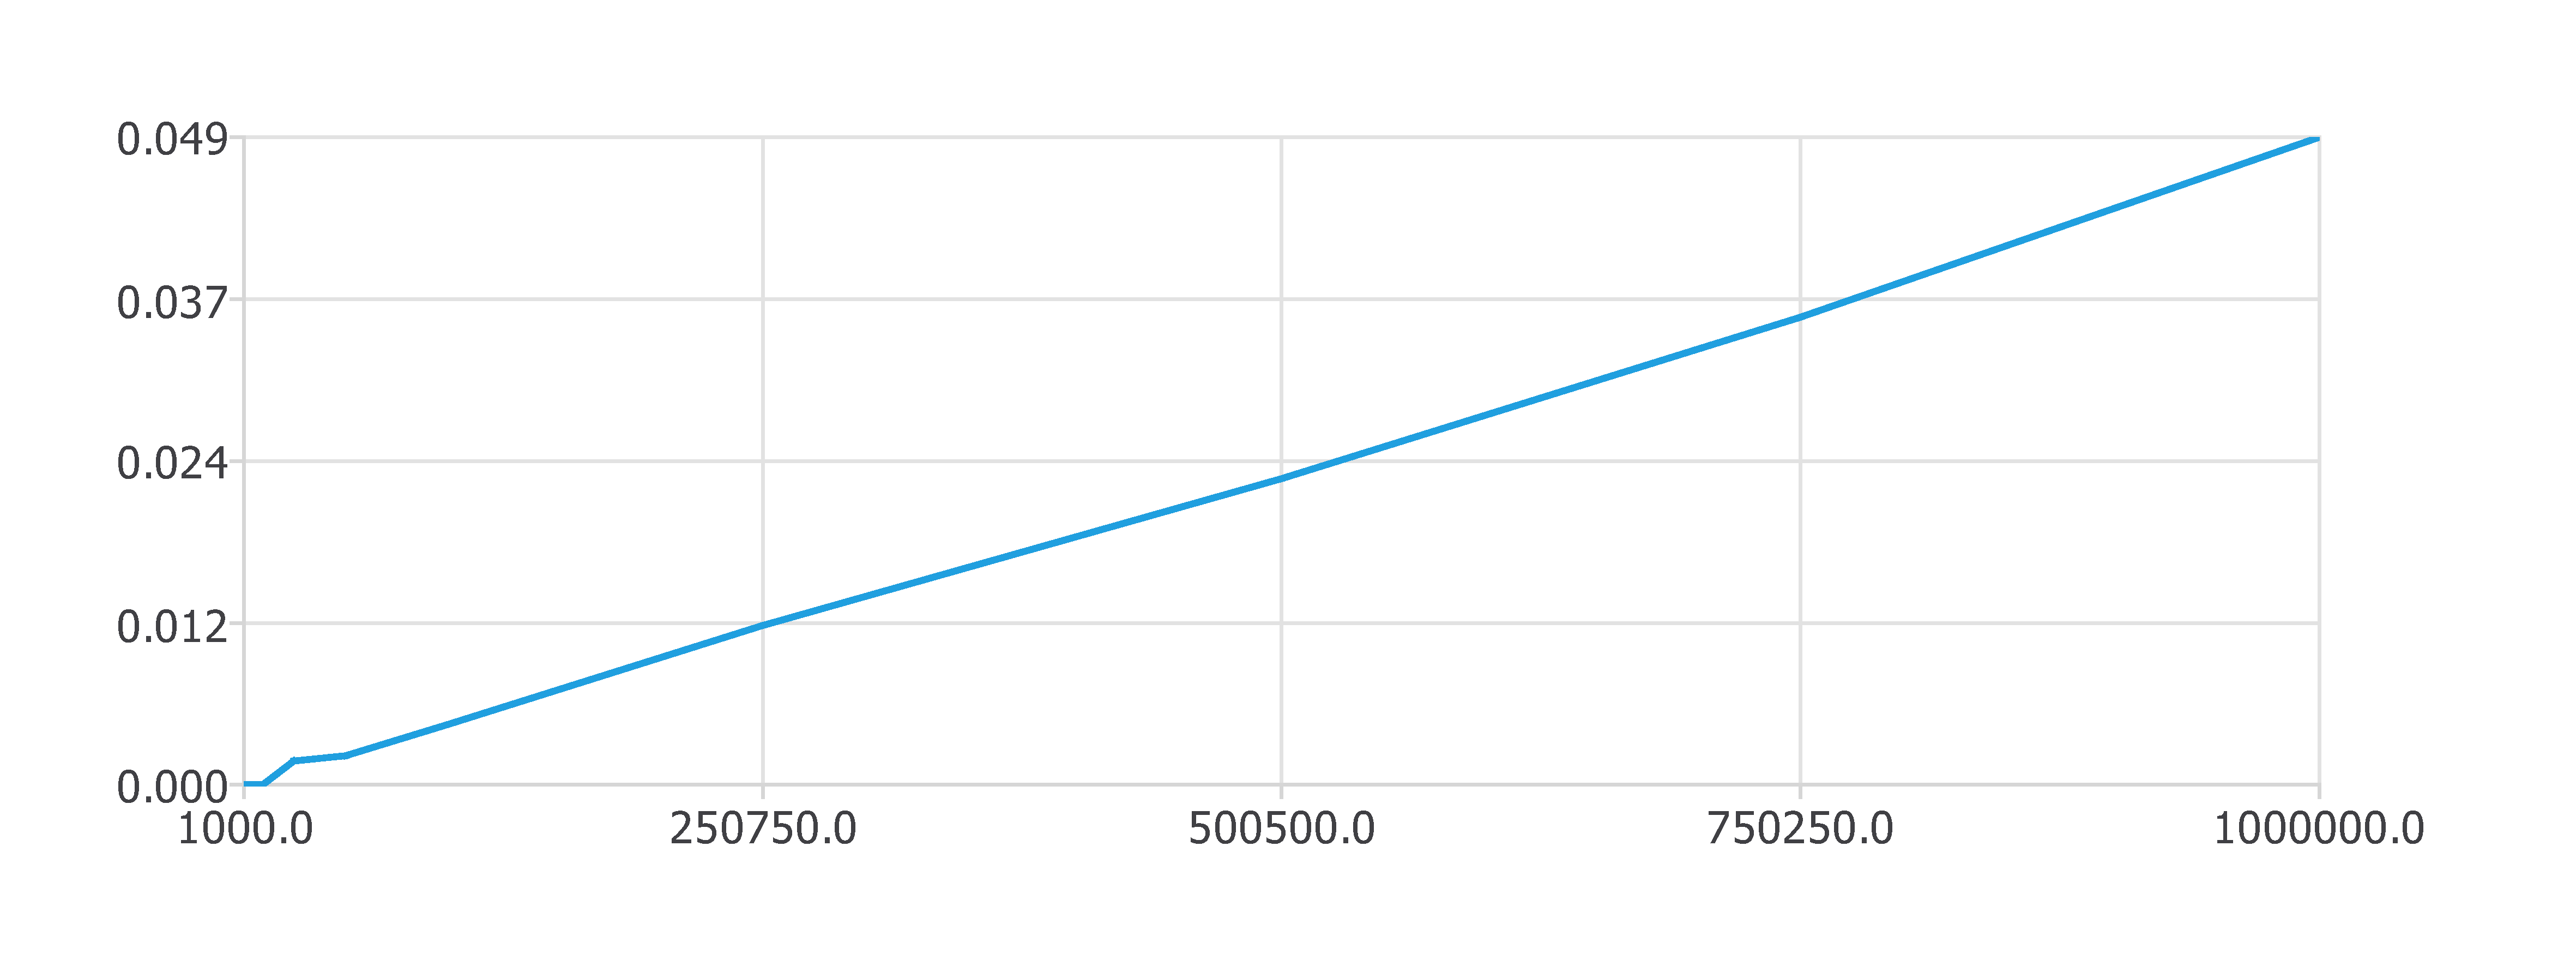
\includegraphics[clip, trim=0cm 0cm 0cm 0cm, width=1\textwidth]{pdf1.pdf}
        \caption{generování jednou}
\end{figure}
\\
\begin{figure}[htbp]
\centering
        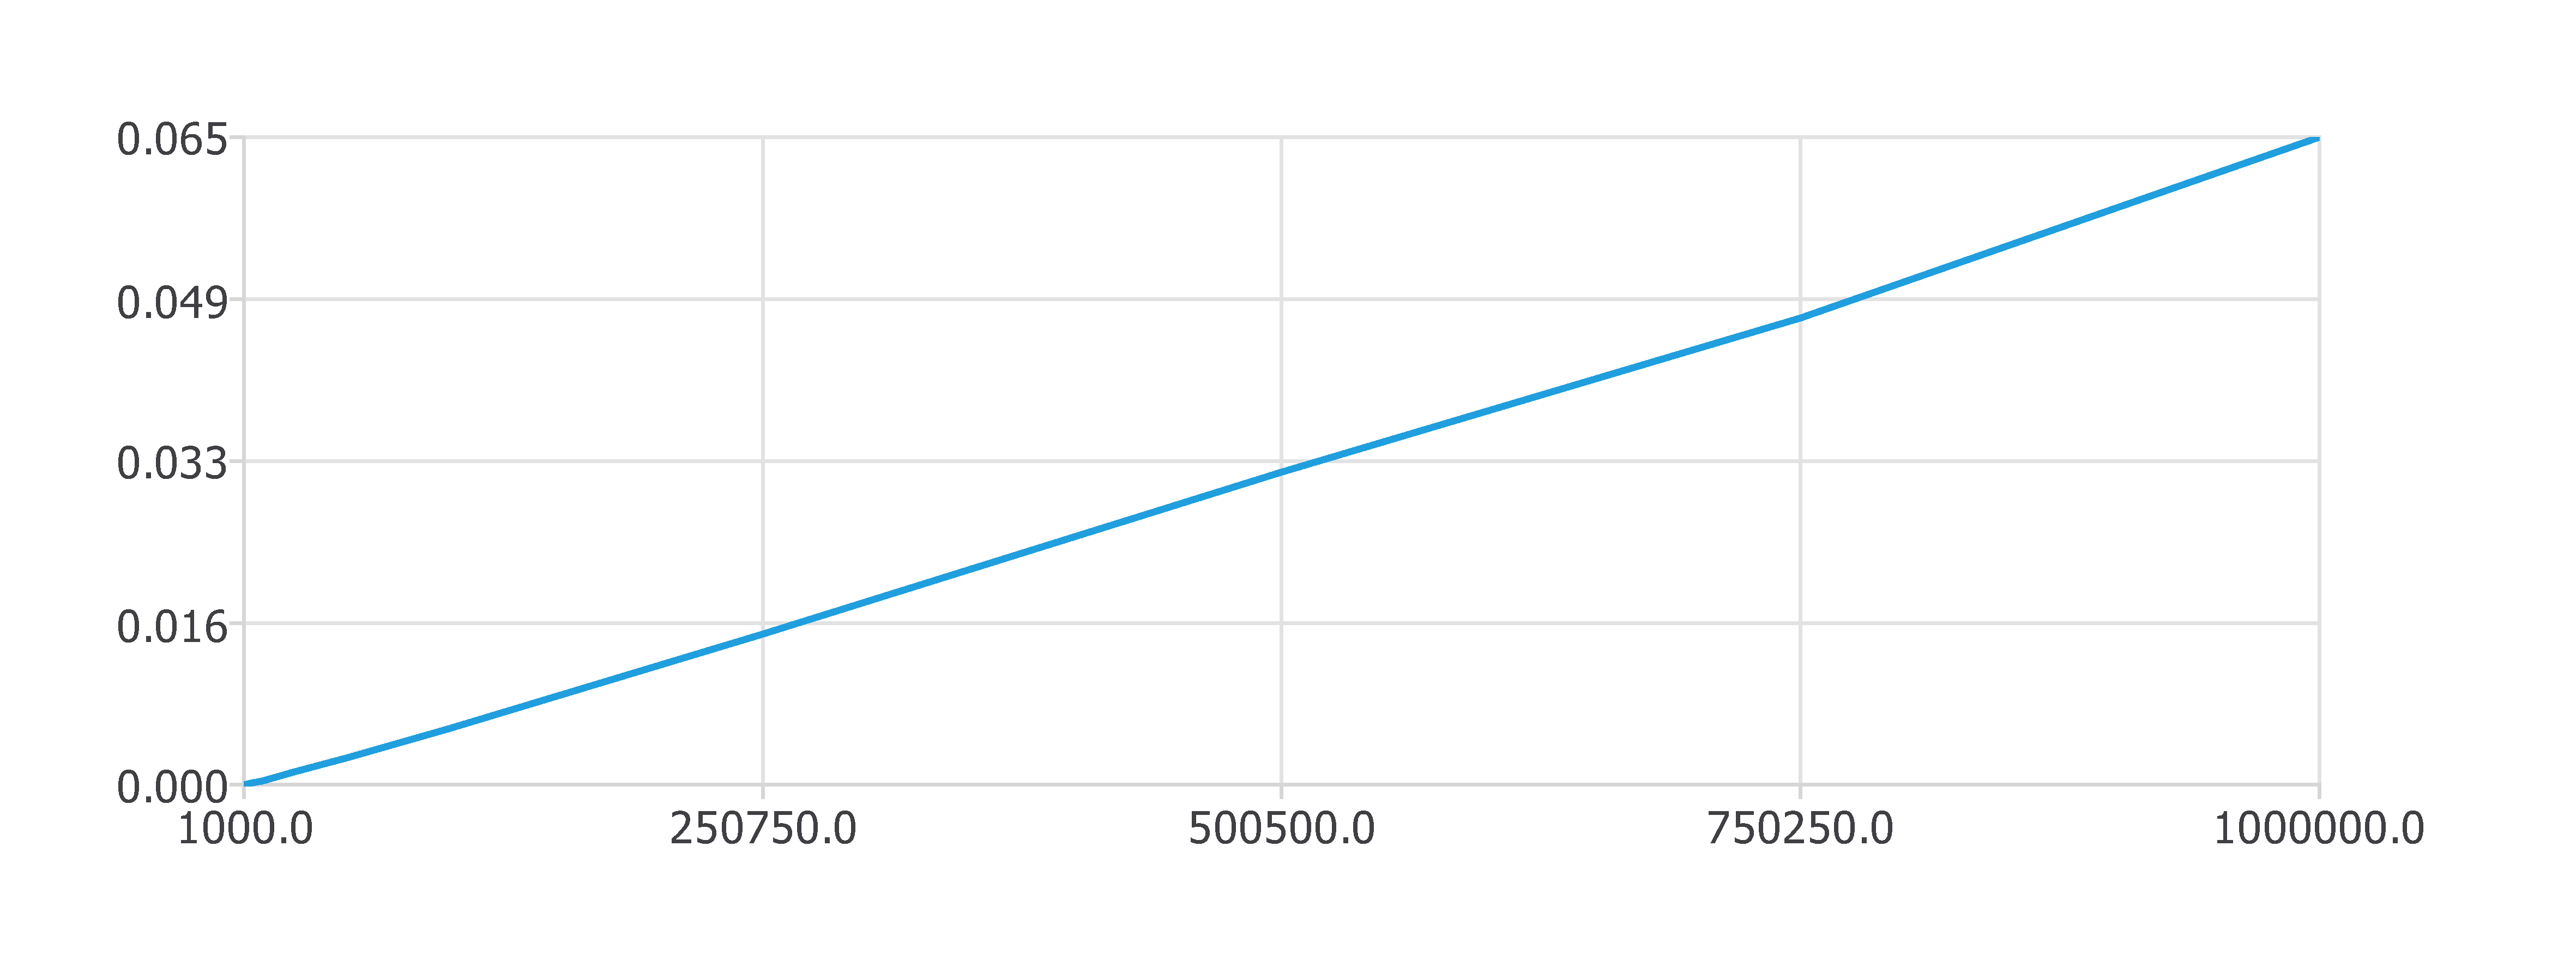
\includegraphics[clip, trim=0cm 0cm 0cm 0cm, width=1\textwidth]{ranj.pdf}
        \caption{generování 10x}
\end{figure}
\clearpage
\newpage
\textit{\textbf {Quick Hull}}
\\
\begin{figure}[htbp]
\centering
        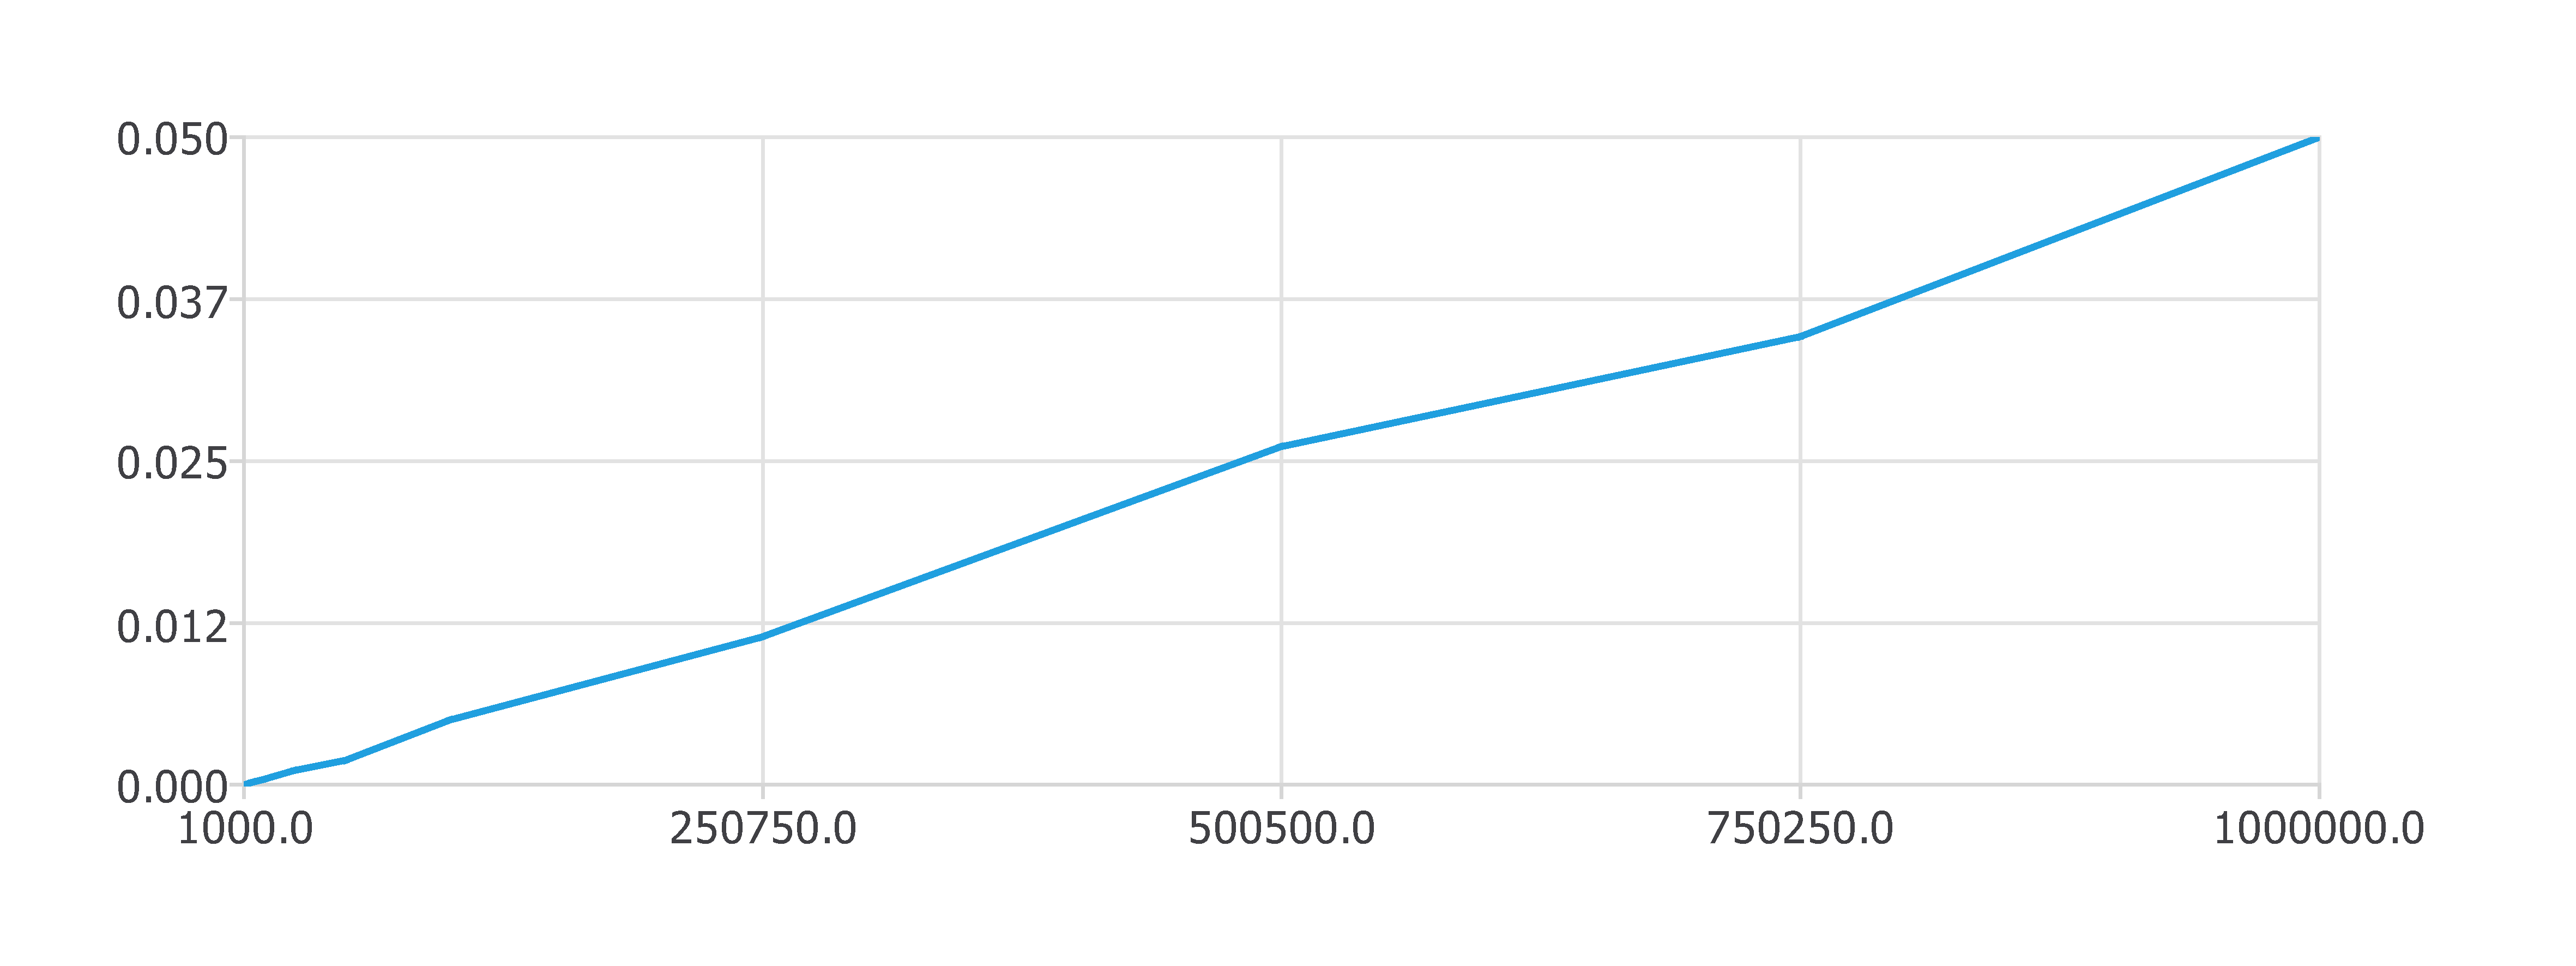
\includegraphics[clip, trim=0cm 0cm 0cm 0cm, width=1\textwidth]{pdf4.pdf}
        \caption{generování}
\end{figure}
\begin{figure}[htbp]
\centering
        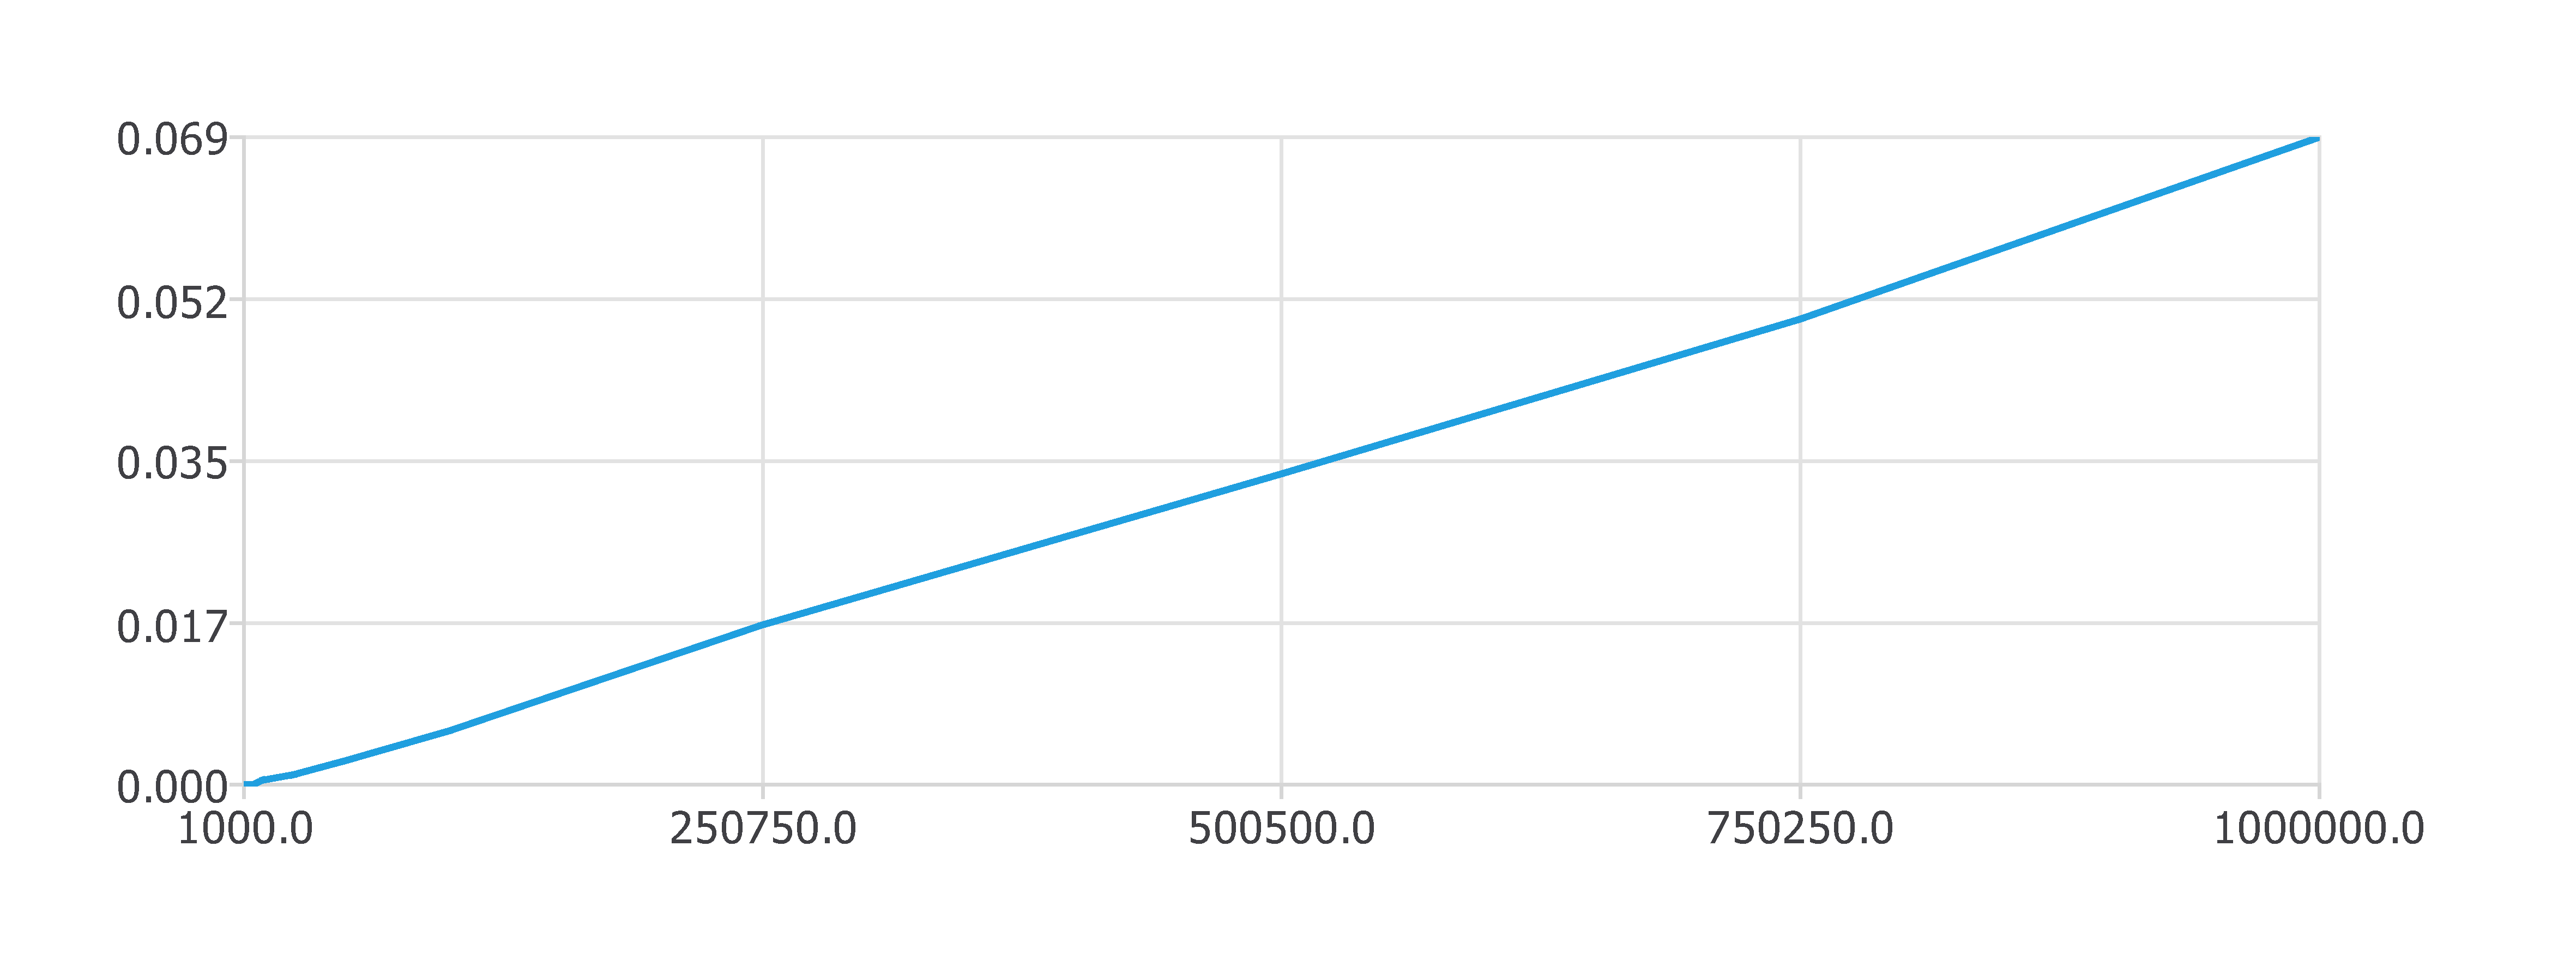
\includegraphics[clip, trim=0cm 0cm 0cm 0cm, width=1\textwidth]{rang.pdf}
        \caption{generování 10x}
\end{figure}
\clearpage
\newpage
\textit{\textbf {Incremental construction}}
\\
\begin{figure}[htbp]
\centering
        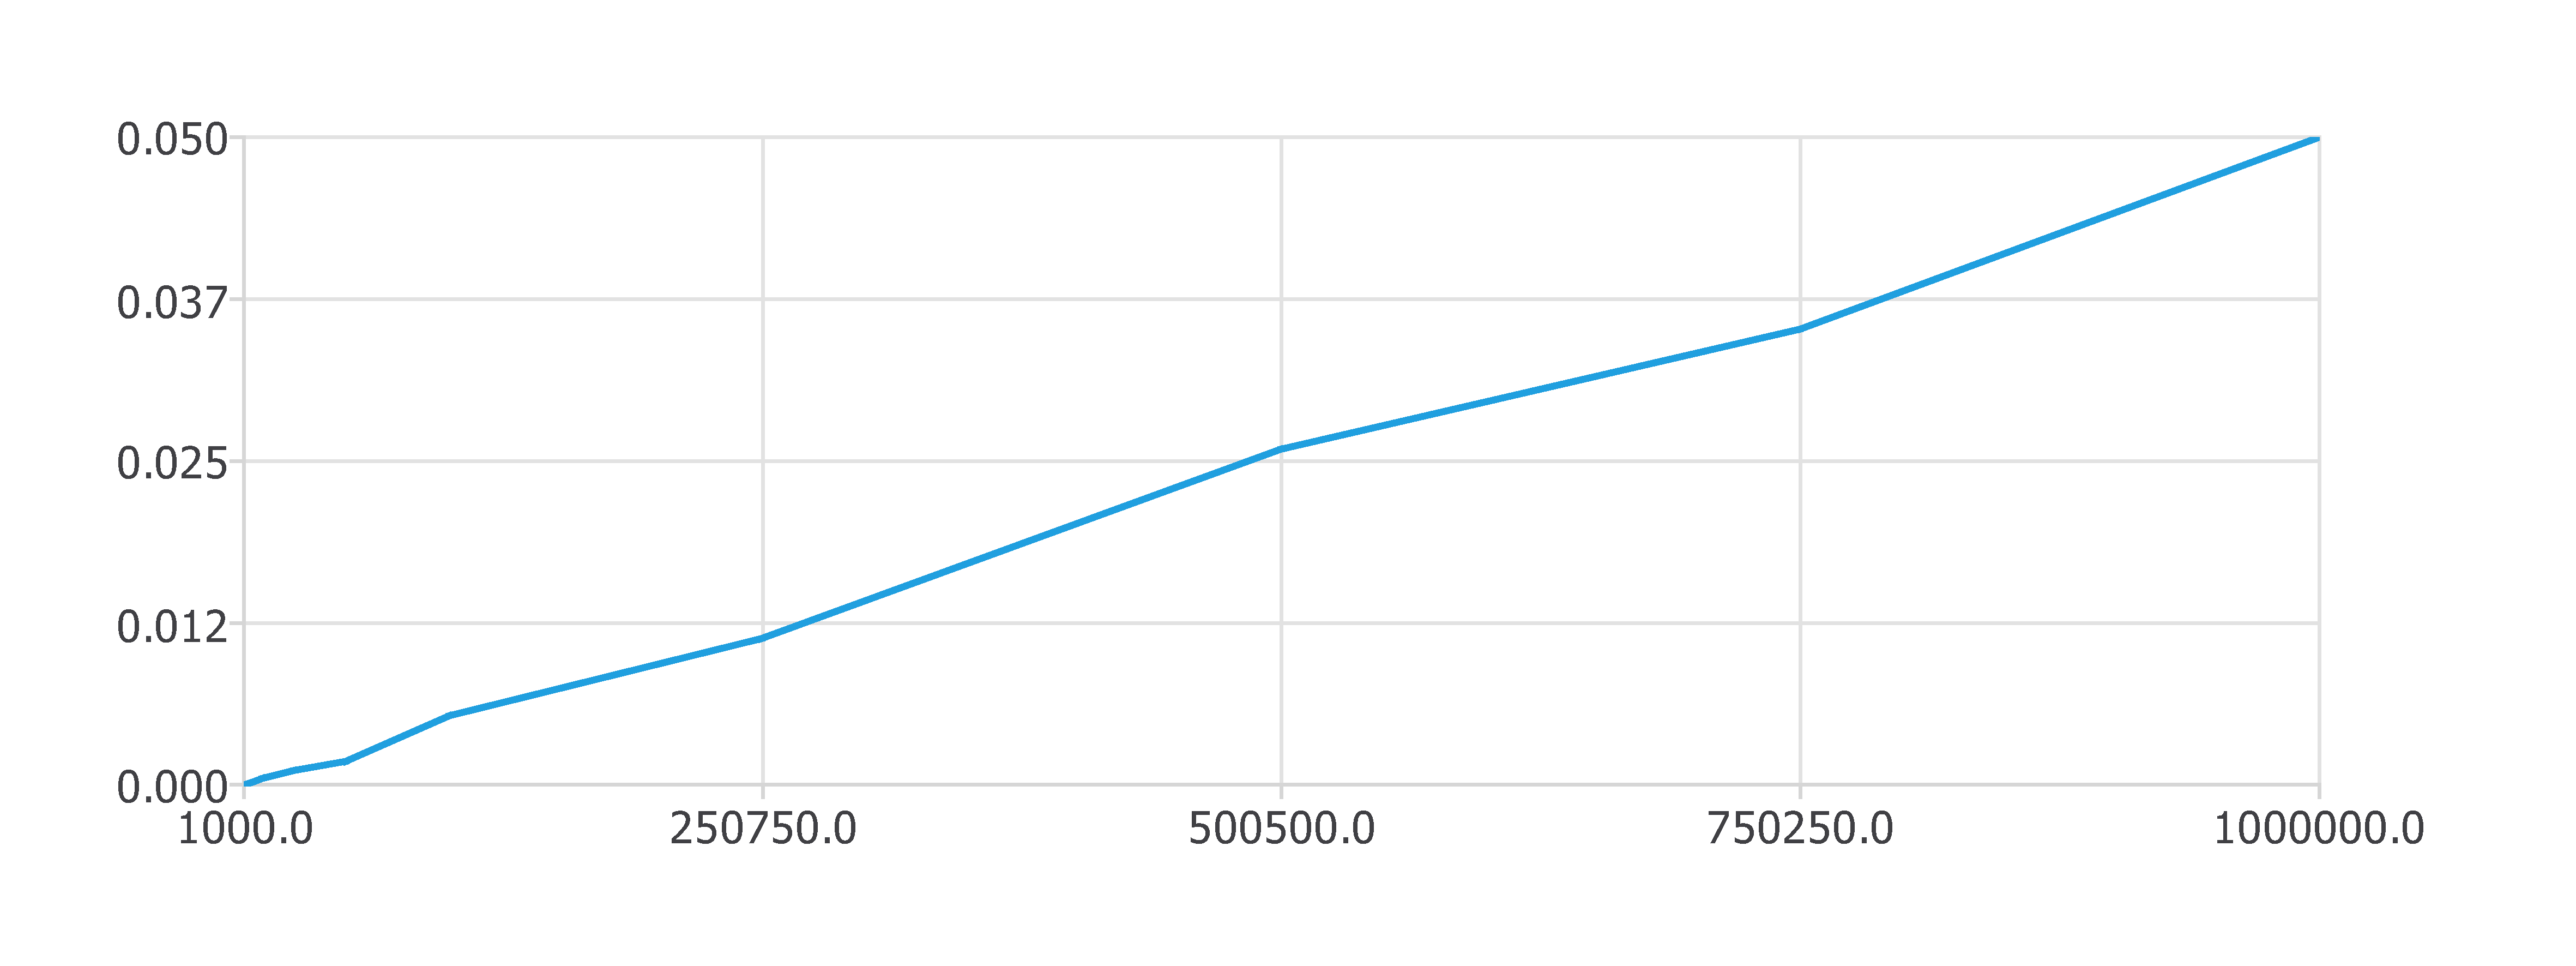
\includegraphics[clip, trim=0cm 0cm 0cm 0cm, width=1\textwidth]{pdf7.pdf}
        \caption{generování}
\end{figure}
\begin{figure}[htbp]
\centering
        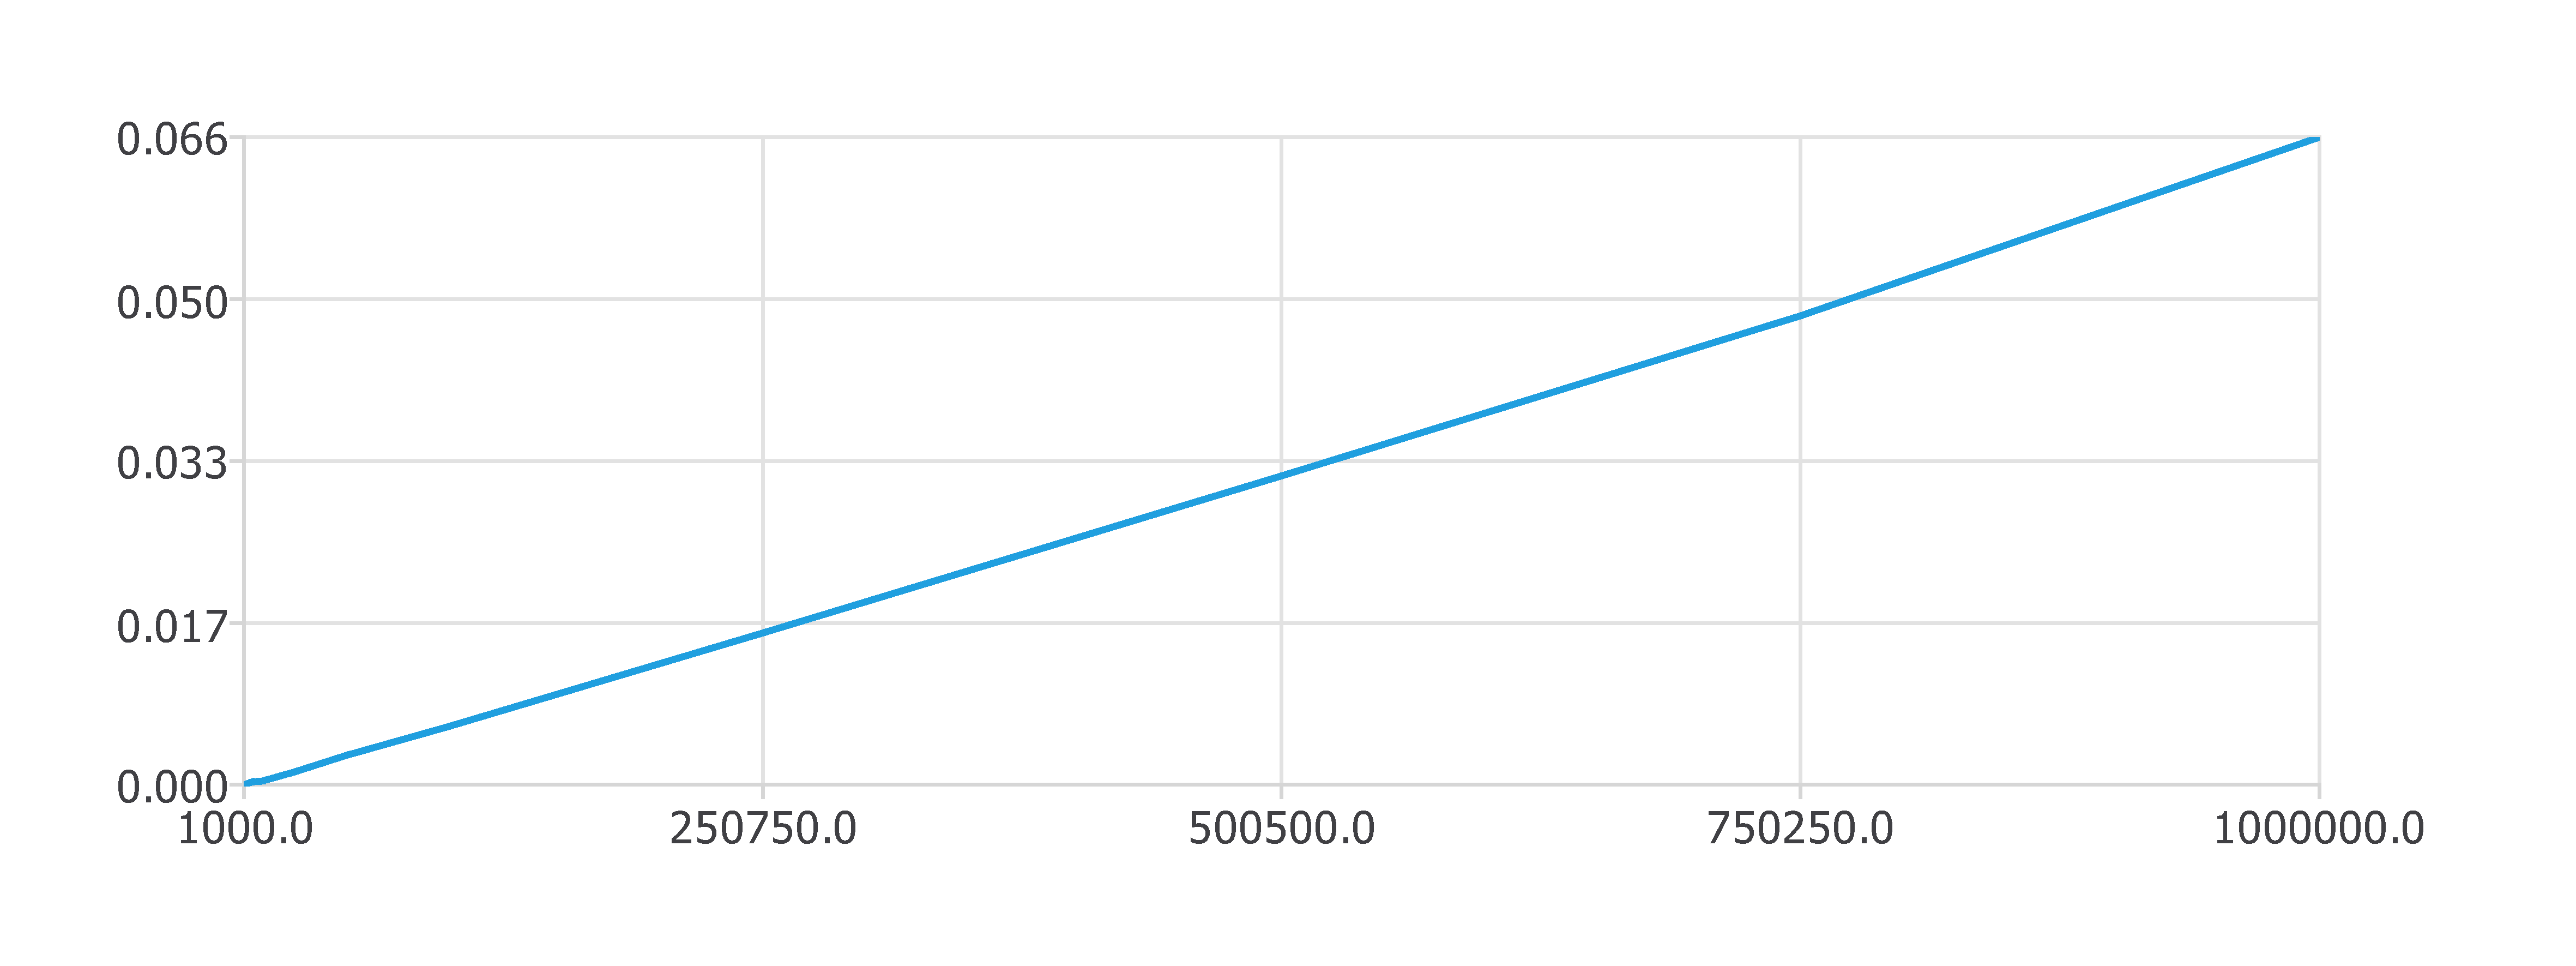
\includegraphics[clip, trim=0cm 0cm 0cm 0cm, width=1\textwidth]{rani.pdf}
        \caption{generování 10x}
\end{figure}
.\\
\clearpage
\newpage
\subsection{GRID}
\textit{\textbf {Jarvis Scan}}
\\
\begin{figure}[htbp]
\centering
        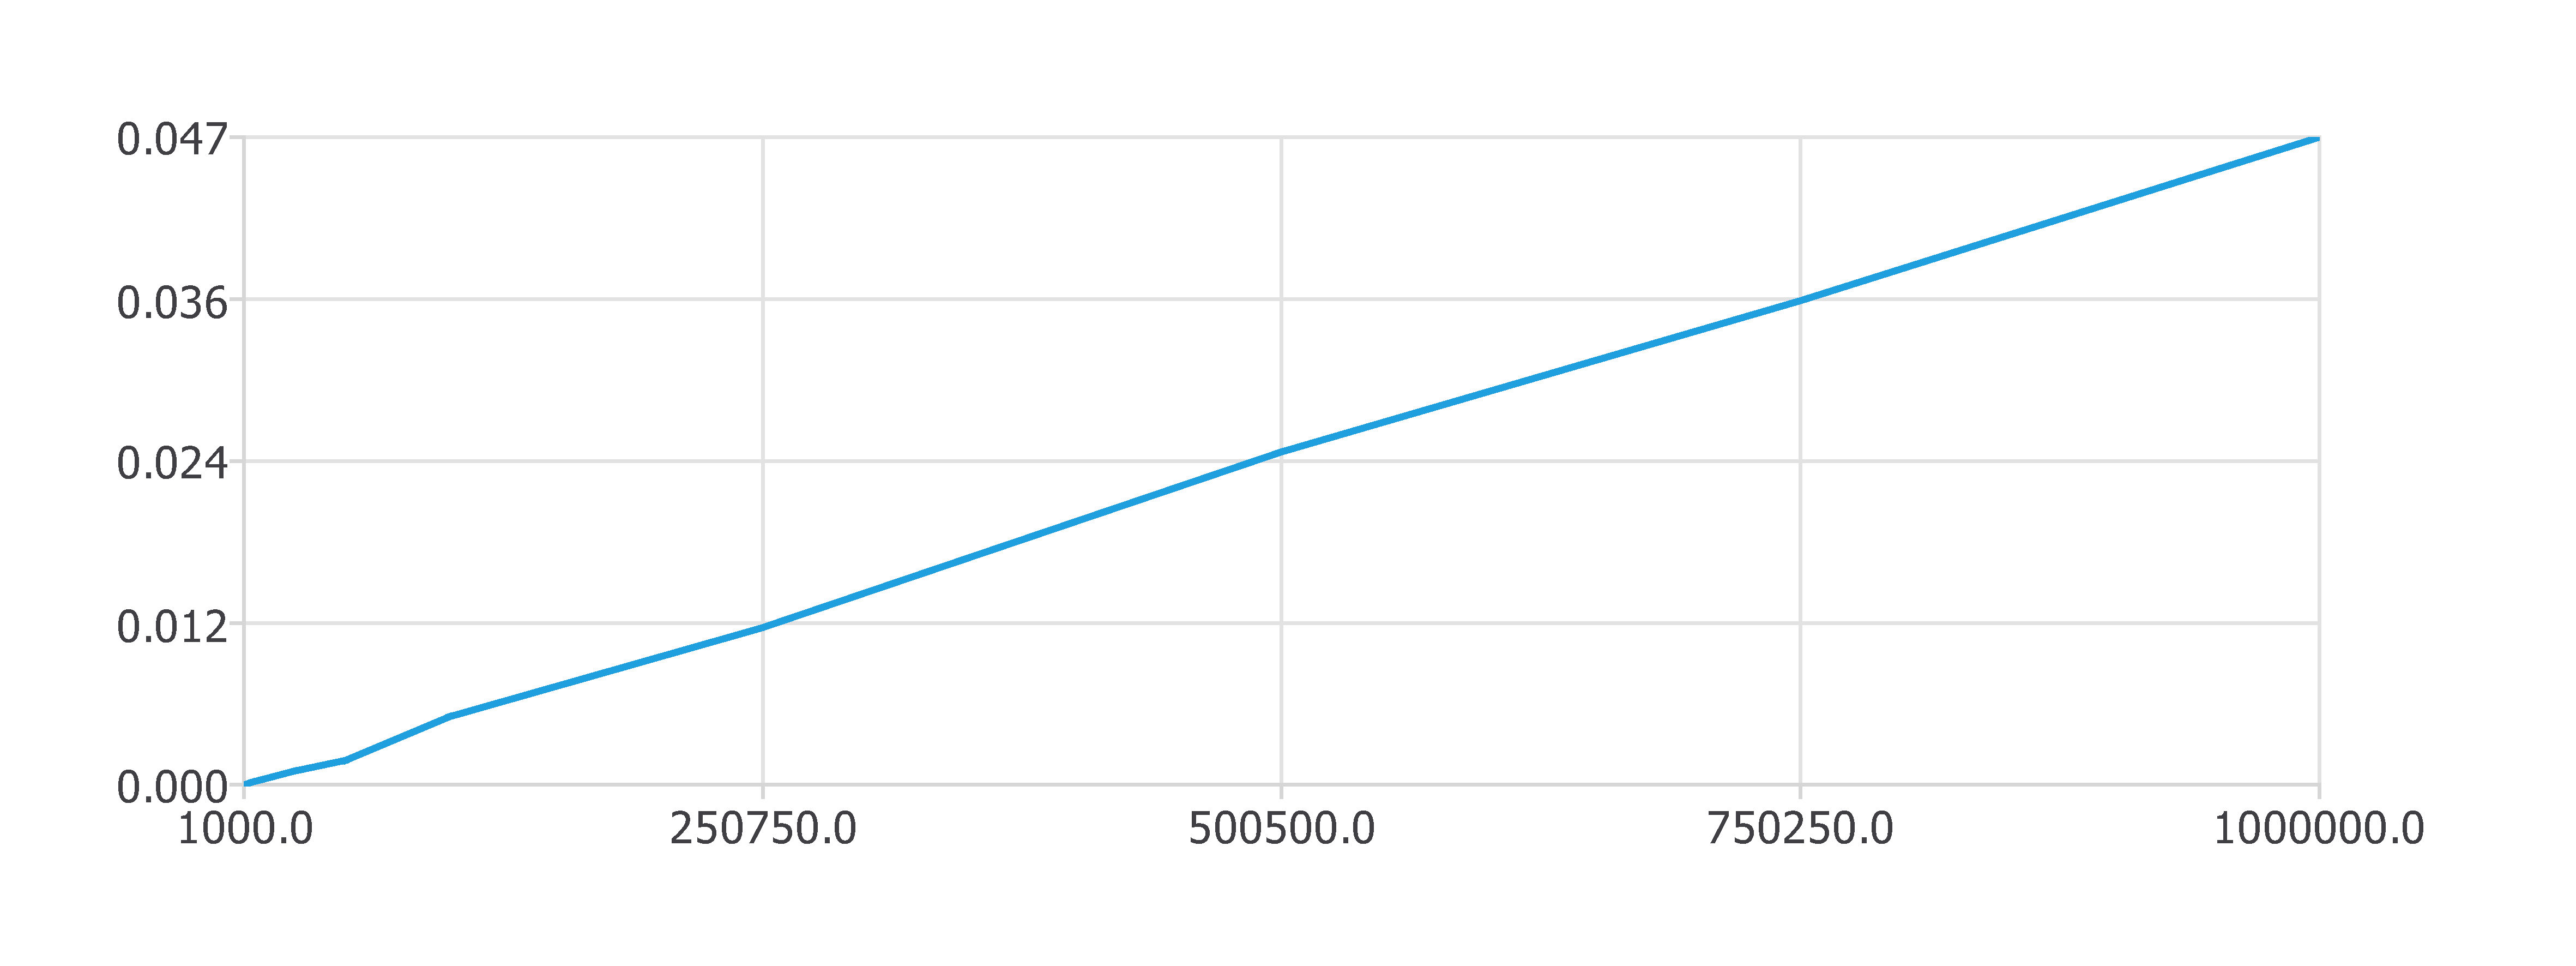
\includegraphics[clip, trim=0cm 0cm 0cm 0cm, width=1\textwidth]{pdf10.pdf}
        \caption{generování}
\end{figure}
\begin{figure}[htbp]
\centering
        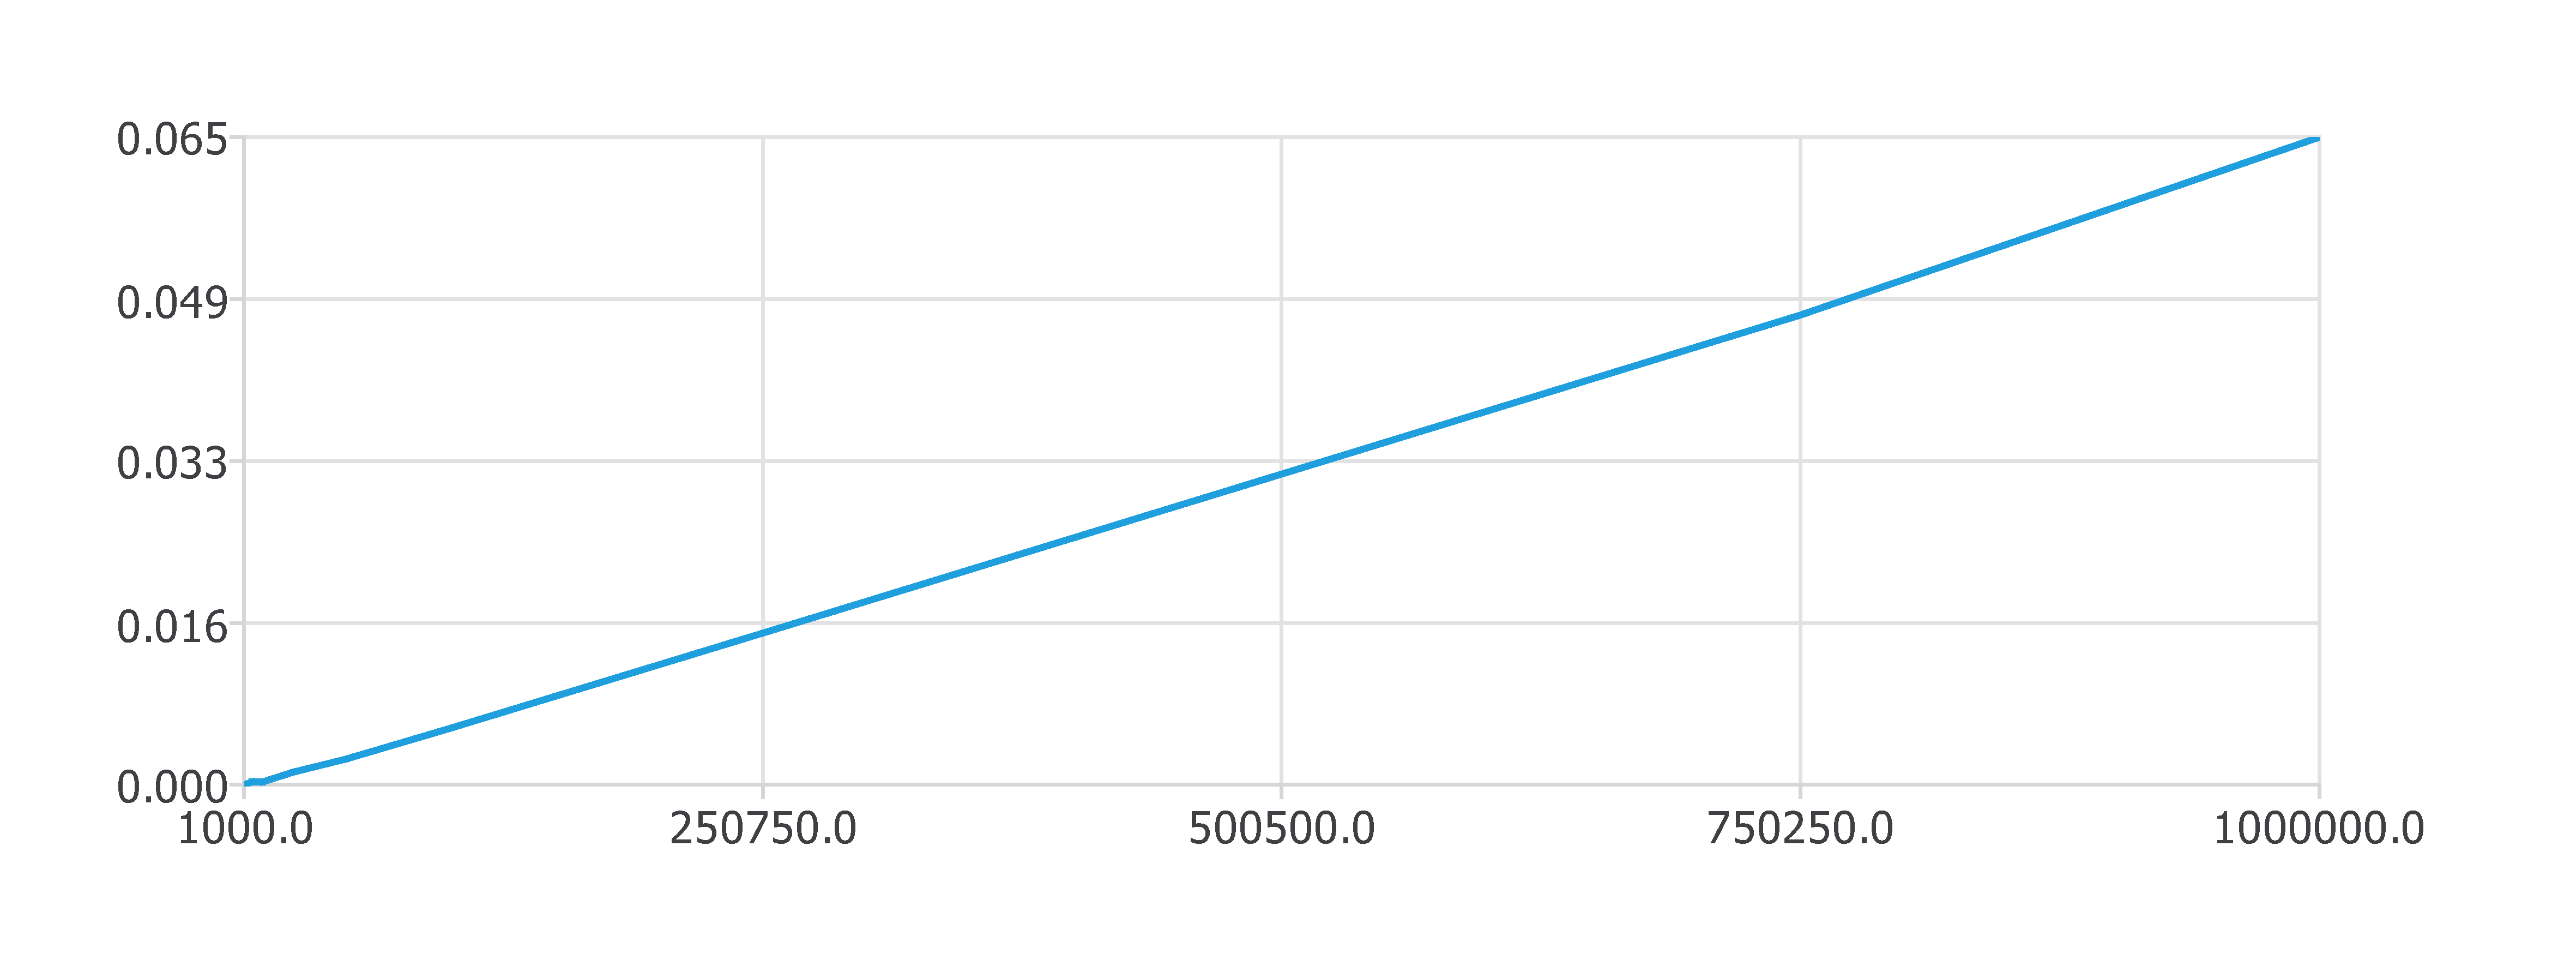
\includegraphics[clip, trim=0cm 0cm 0cm 0cm, width=1\textwidth]{grj.pdf}
        \caption{generování 10x}
\end{figure}
\\
\clearpage
\newpage
\textit{\textbf {Quick Hull}}
\\
\begin{figure}[htbp]
\centering
        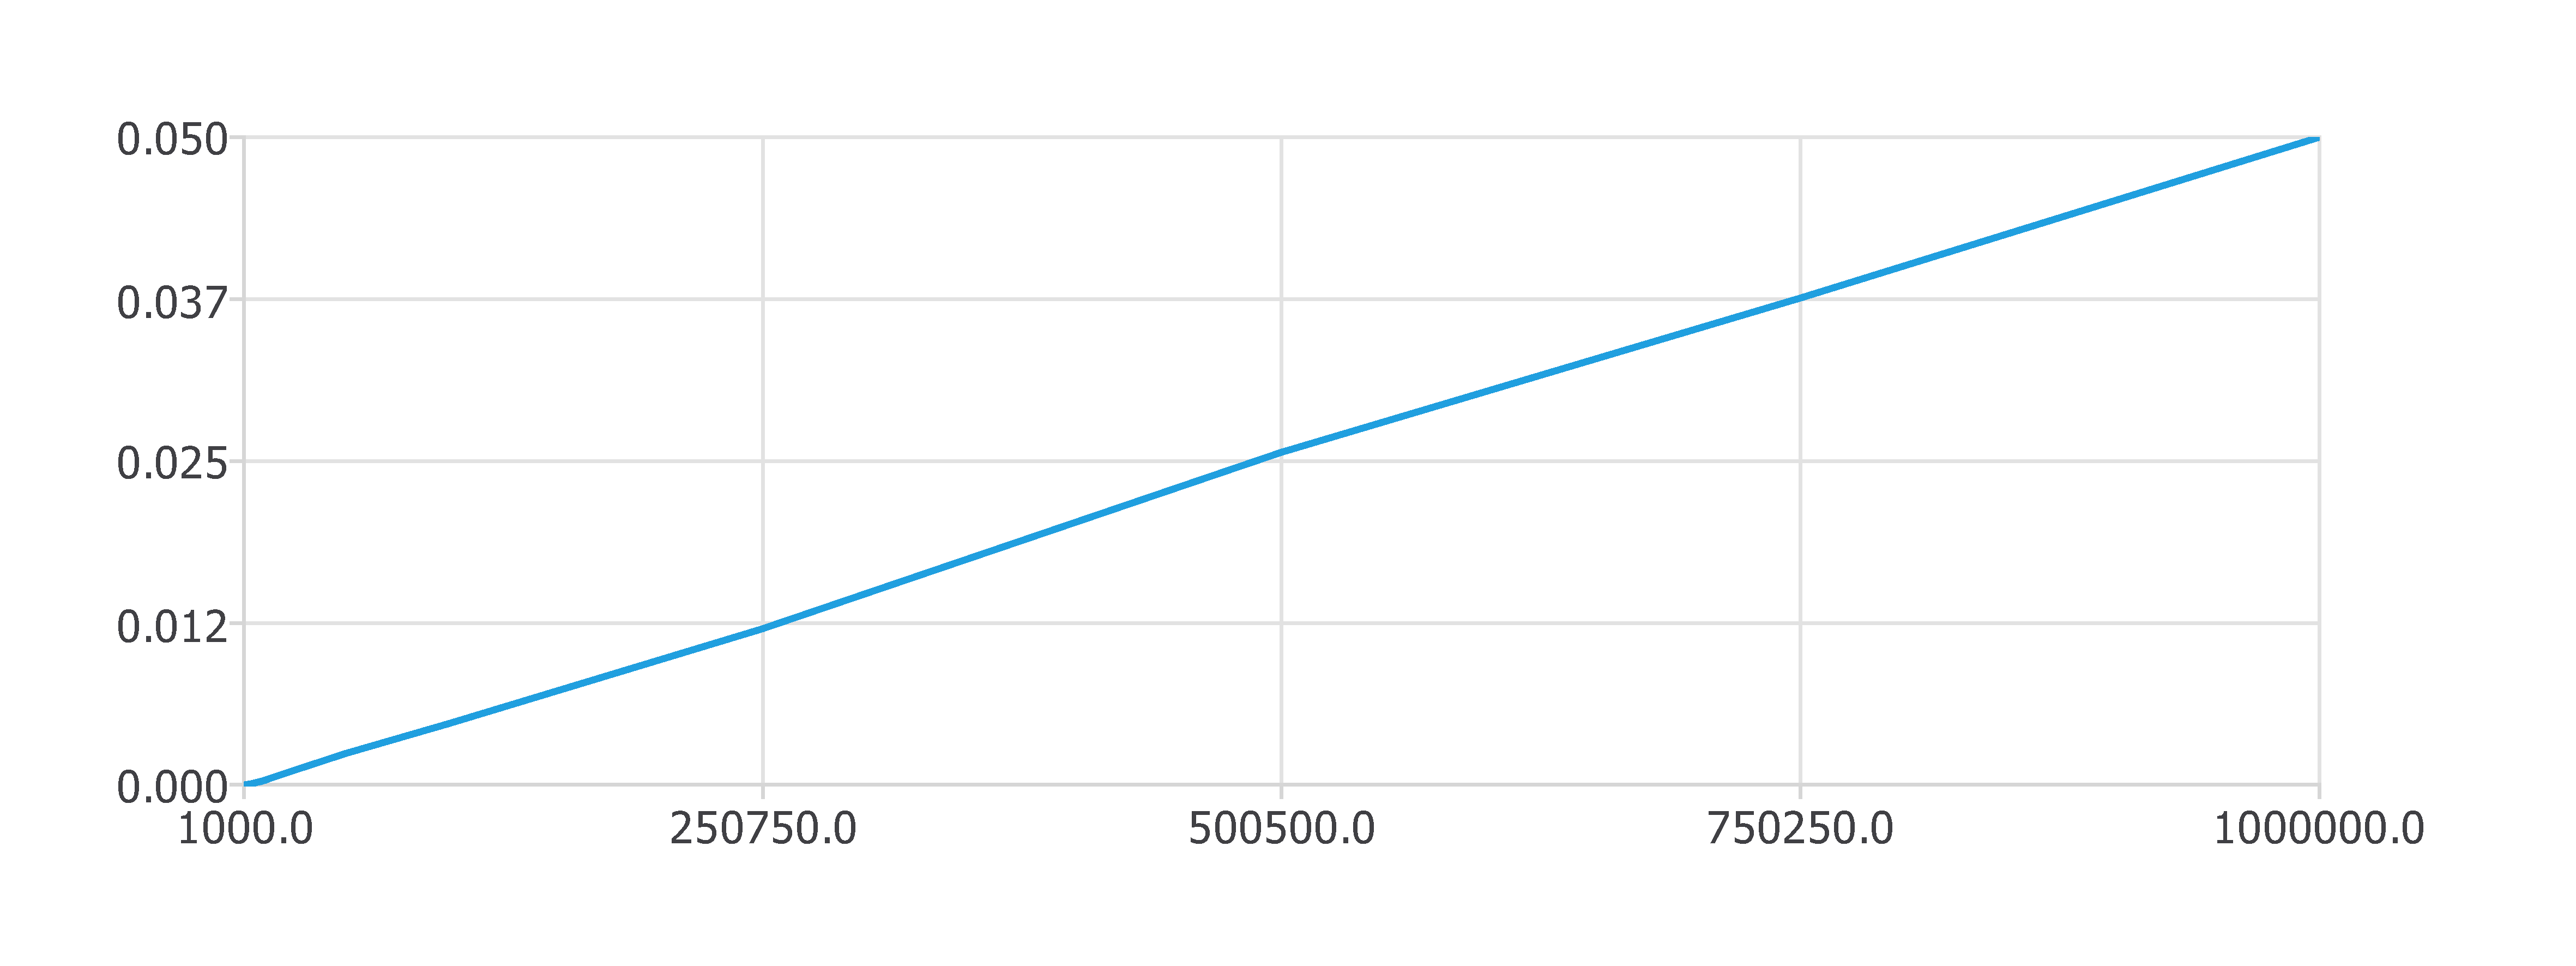
\includegraphics[clip, trim=0cm 0cm 0cm 0cm, width=1\textwidth]{pdf13.pdf}
        \caption{generování}
\end{figure}
\begin{figure}[htbp]
\centering
        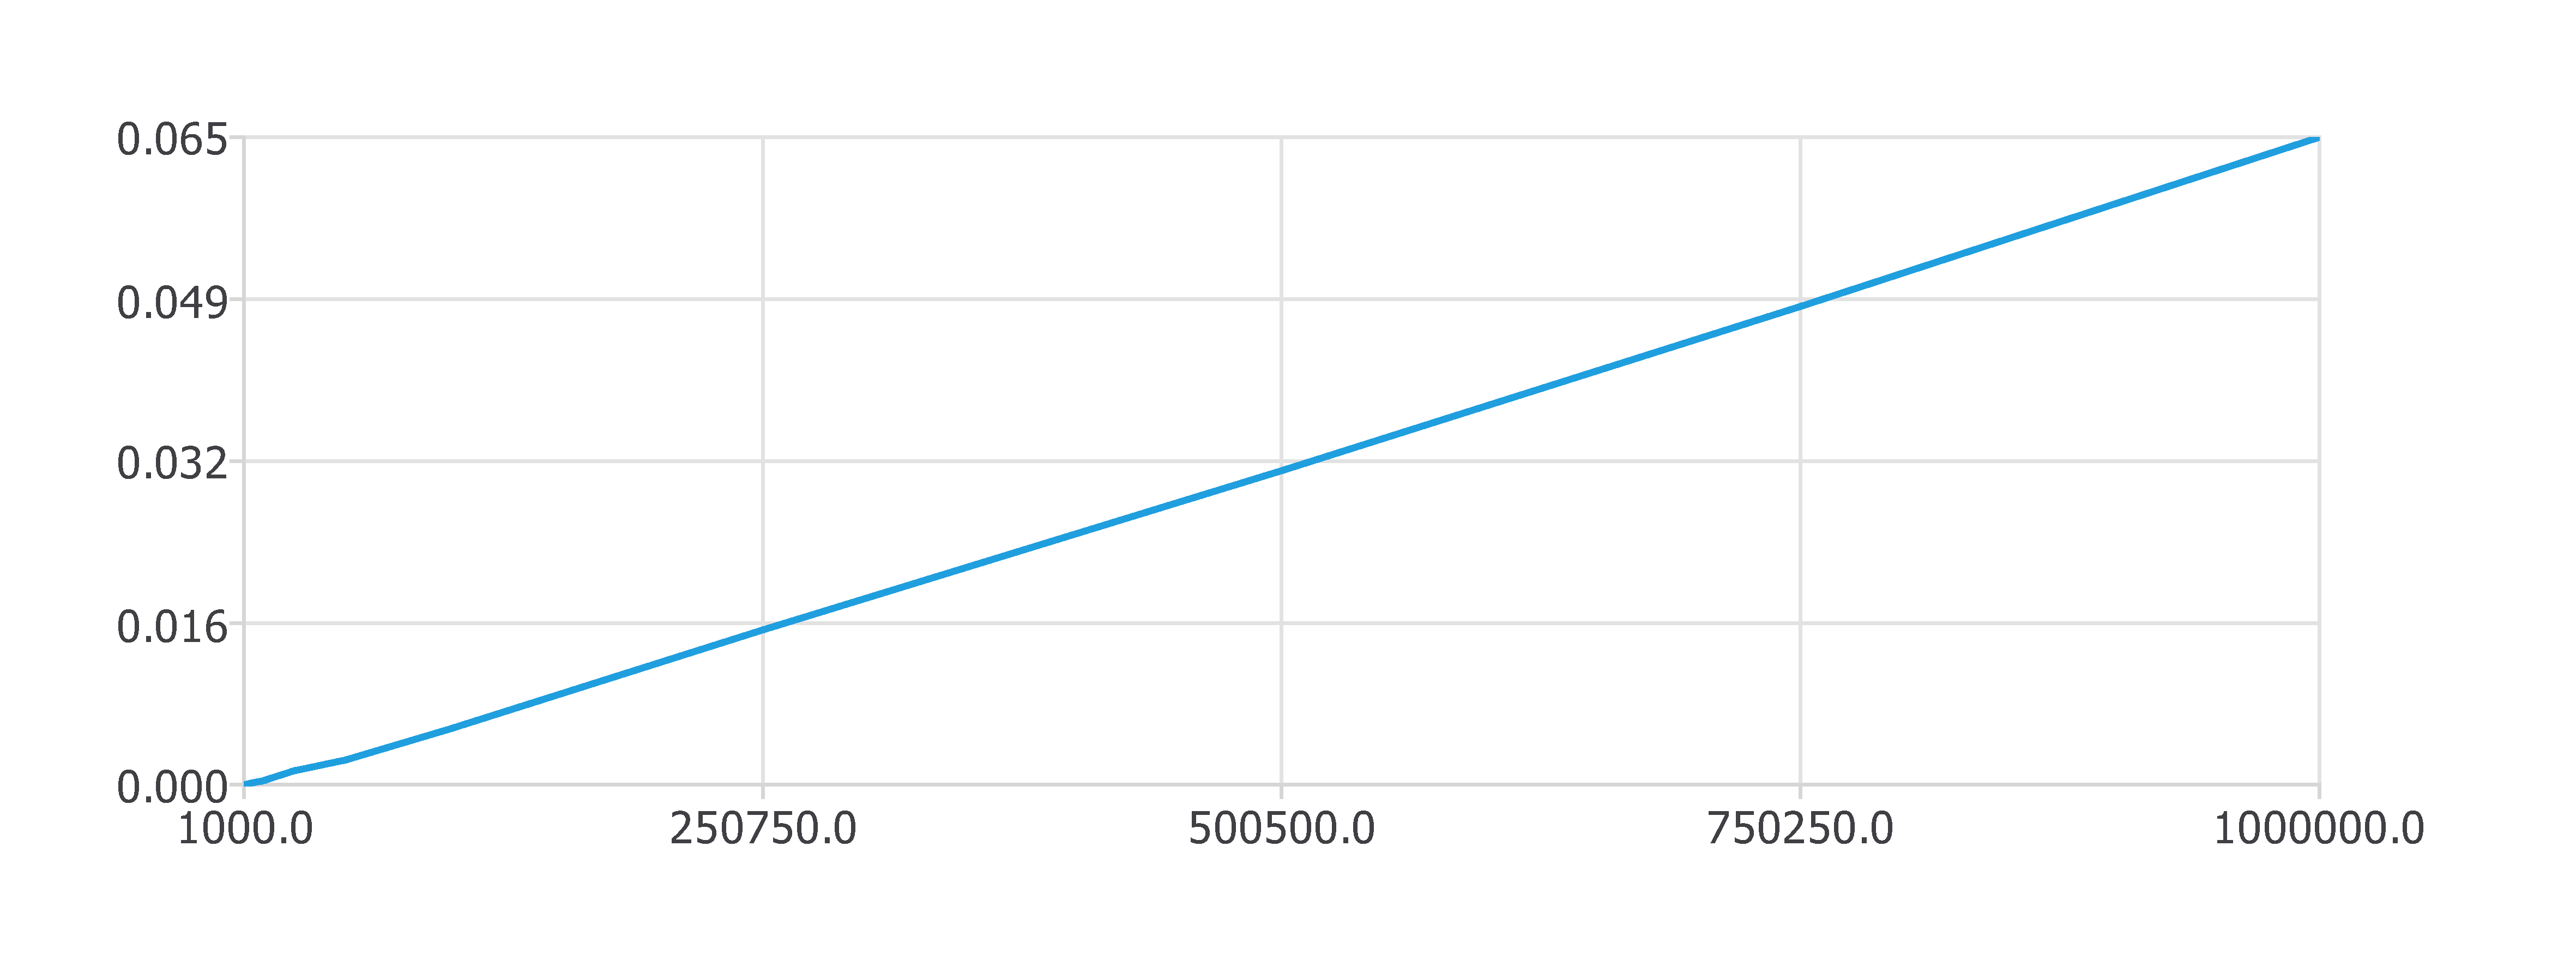
\includegraphics[clip, trim=0cm 0cm 0cm 0cm, width=1\textwidth]{grq.pdf}
        \caption{generování 10x}
\end{figure}
\clearpage
\newpage
\textit{\textbf {Incremental construction}}
\\
\begin{figure}[htbp]
\centering
        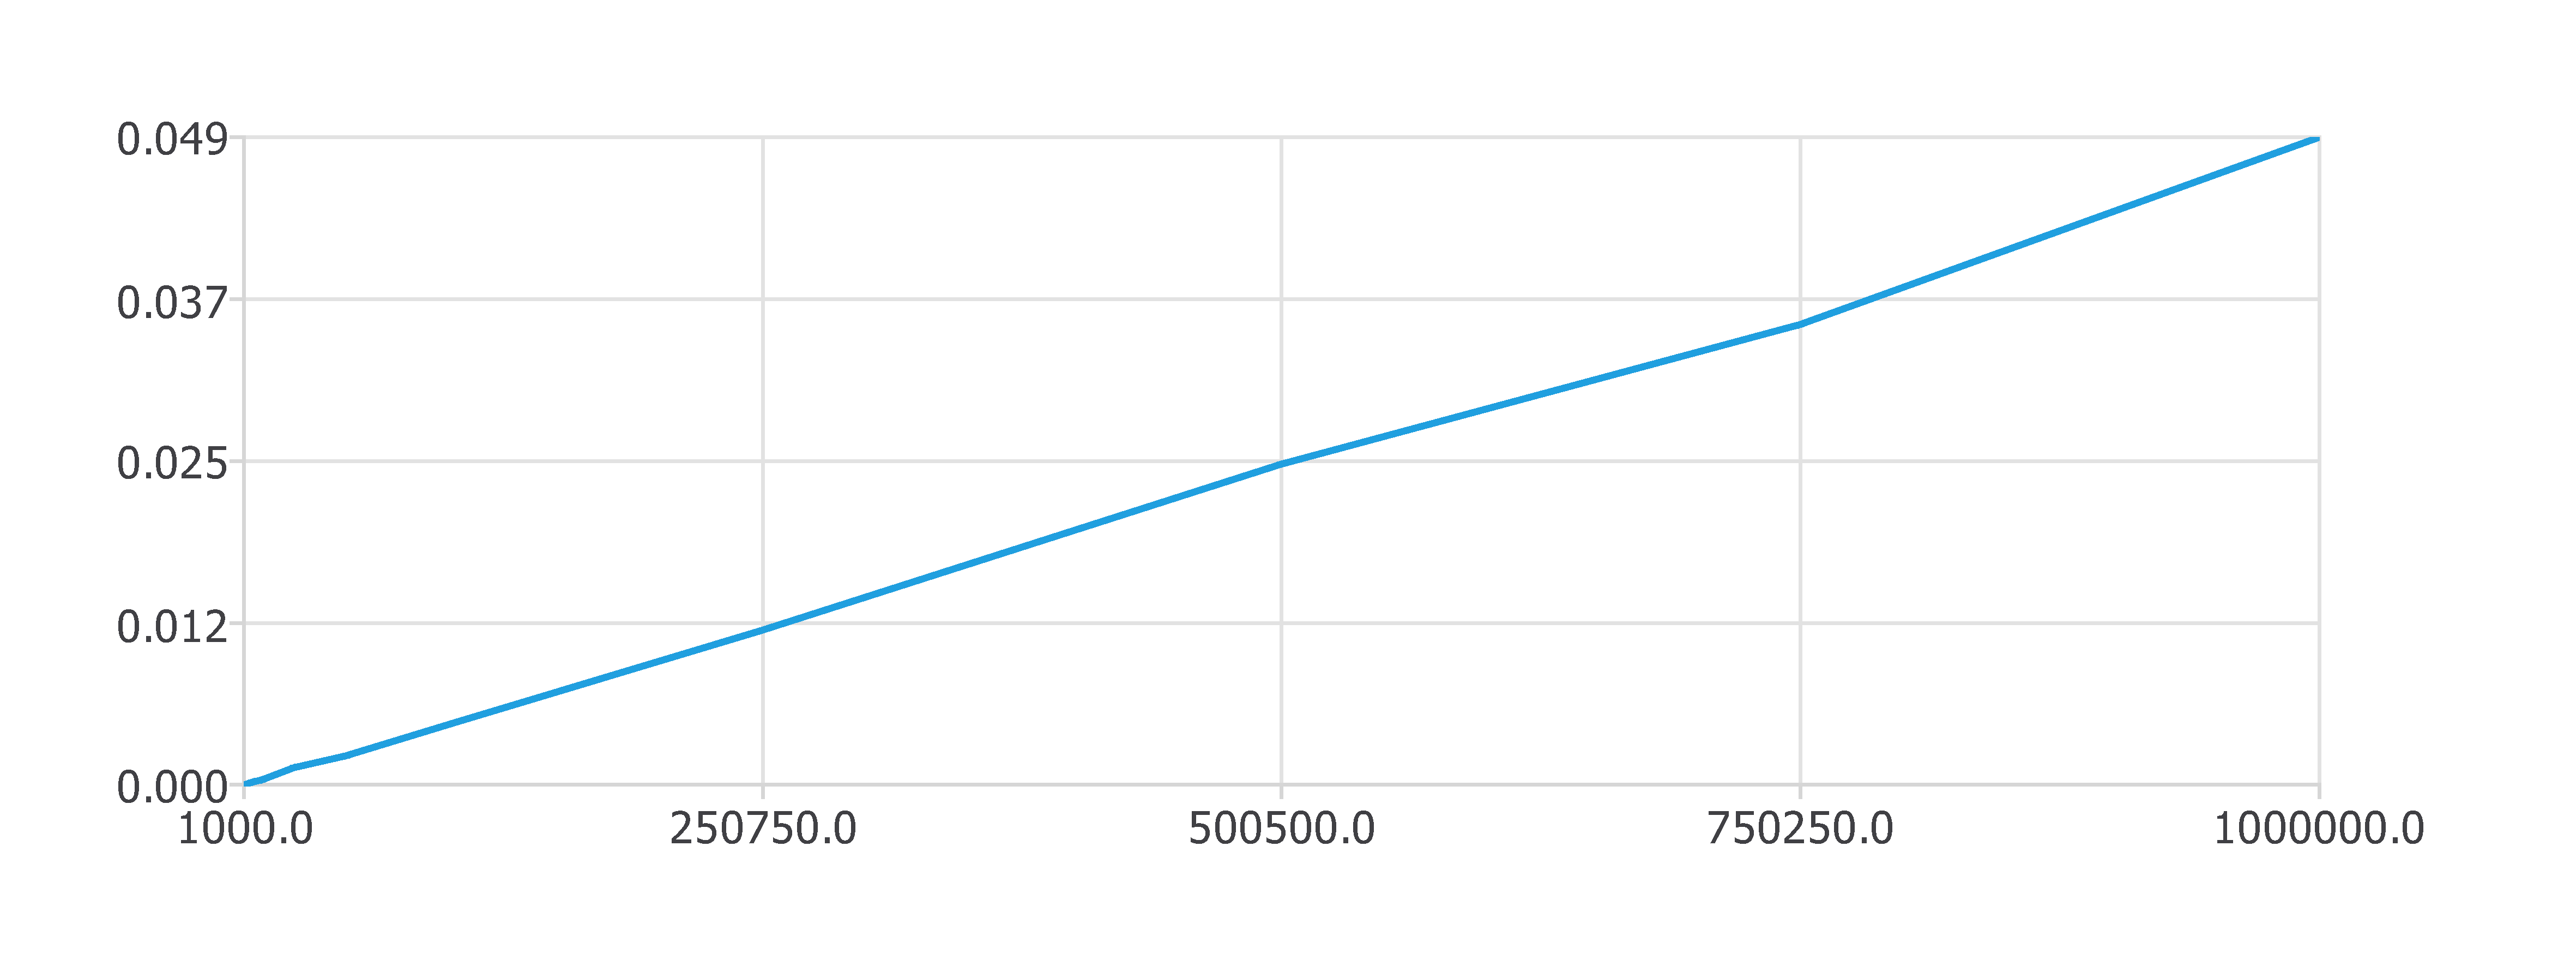
\includegraphics[clip, trim=0cm 0cm 0cm 0cm, width=1\textwidth]{pdf16.pdf}
        \caption{generování}
\end{figure}
\begin{figure}[htbp]
\centering
        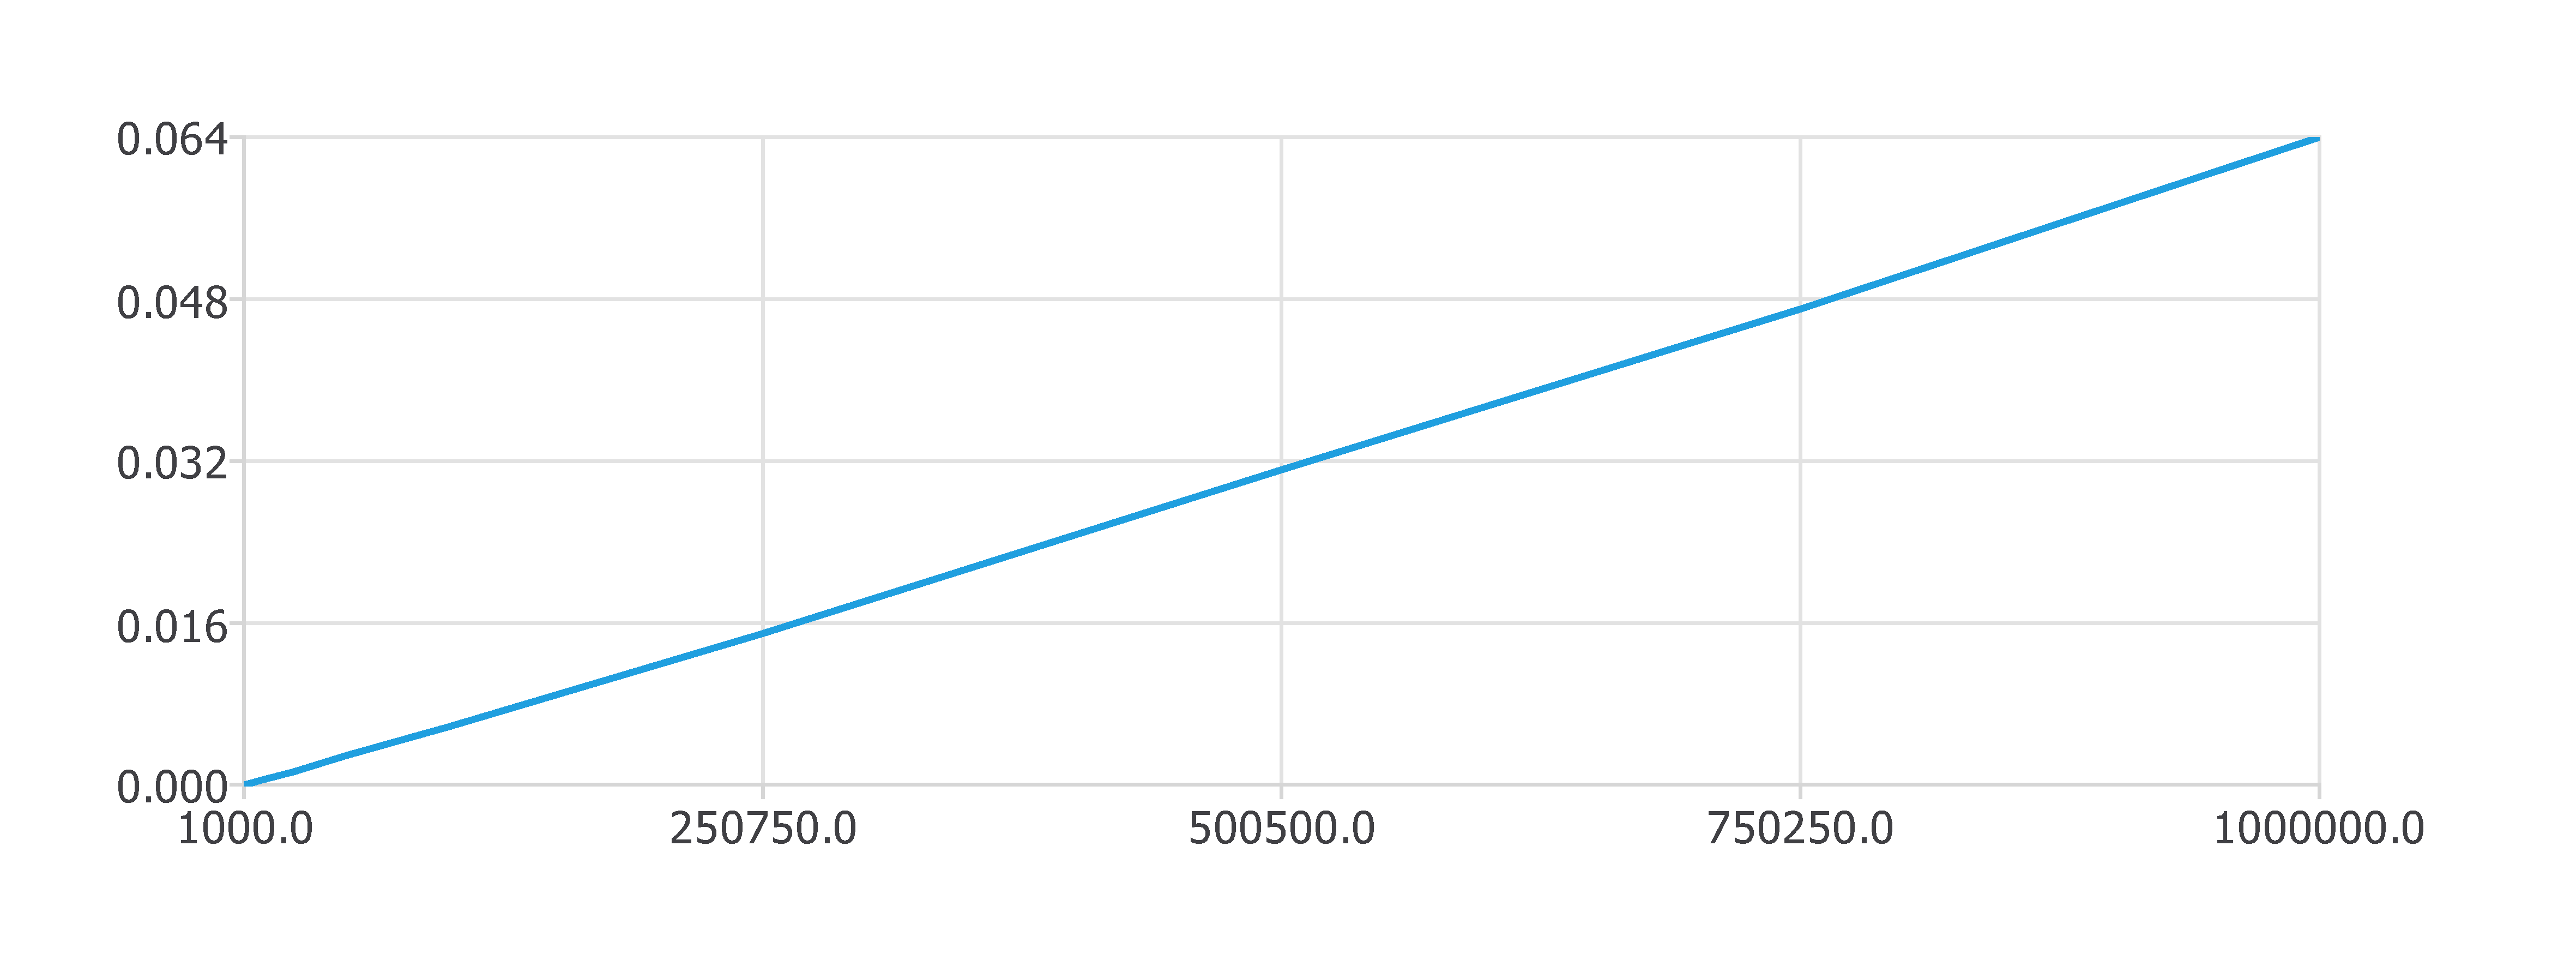
\includegraphics[clip, trim=0cm 0cm 0cm 0cm, width=1\textwidth]{gri.pdf}
        \caption{generování 10x}
\end{figure}
.\\
\bigskip
\clearpage
\newpage
\subsection{CLUSTER}
\textit{\textbf {Jarvis Scan}}
\\
\begin{figure}[htbp]
\centering
        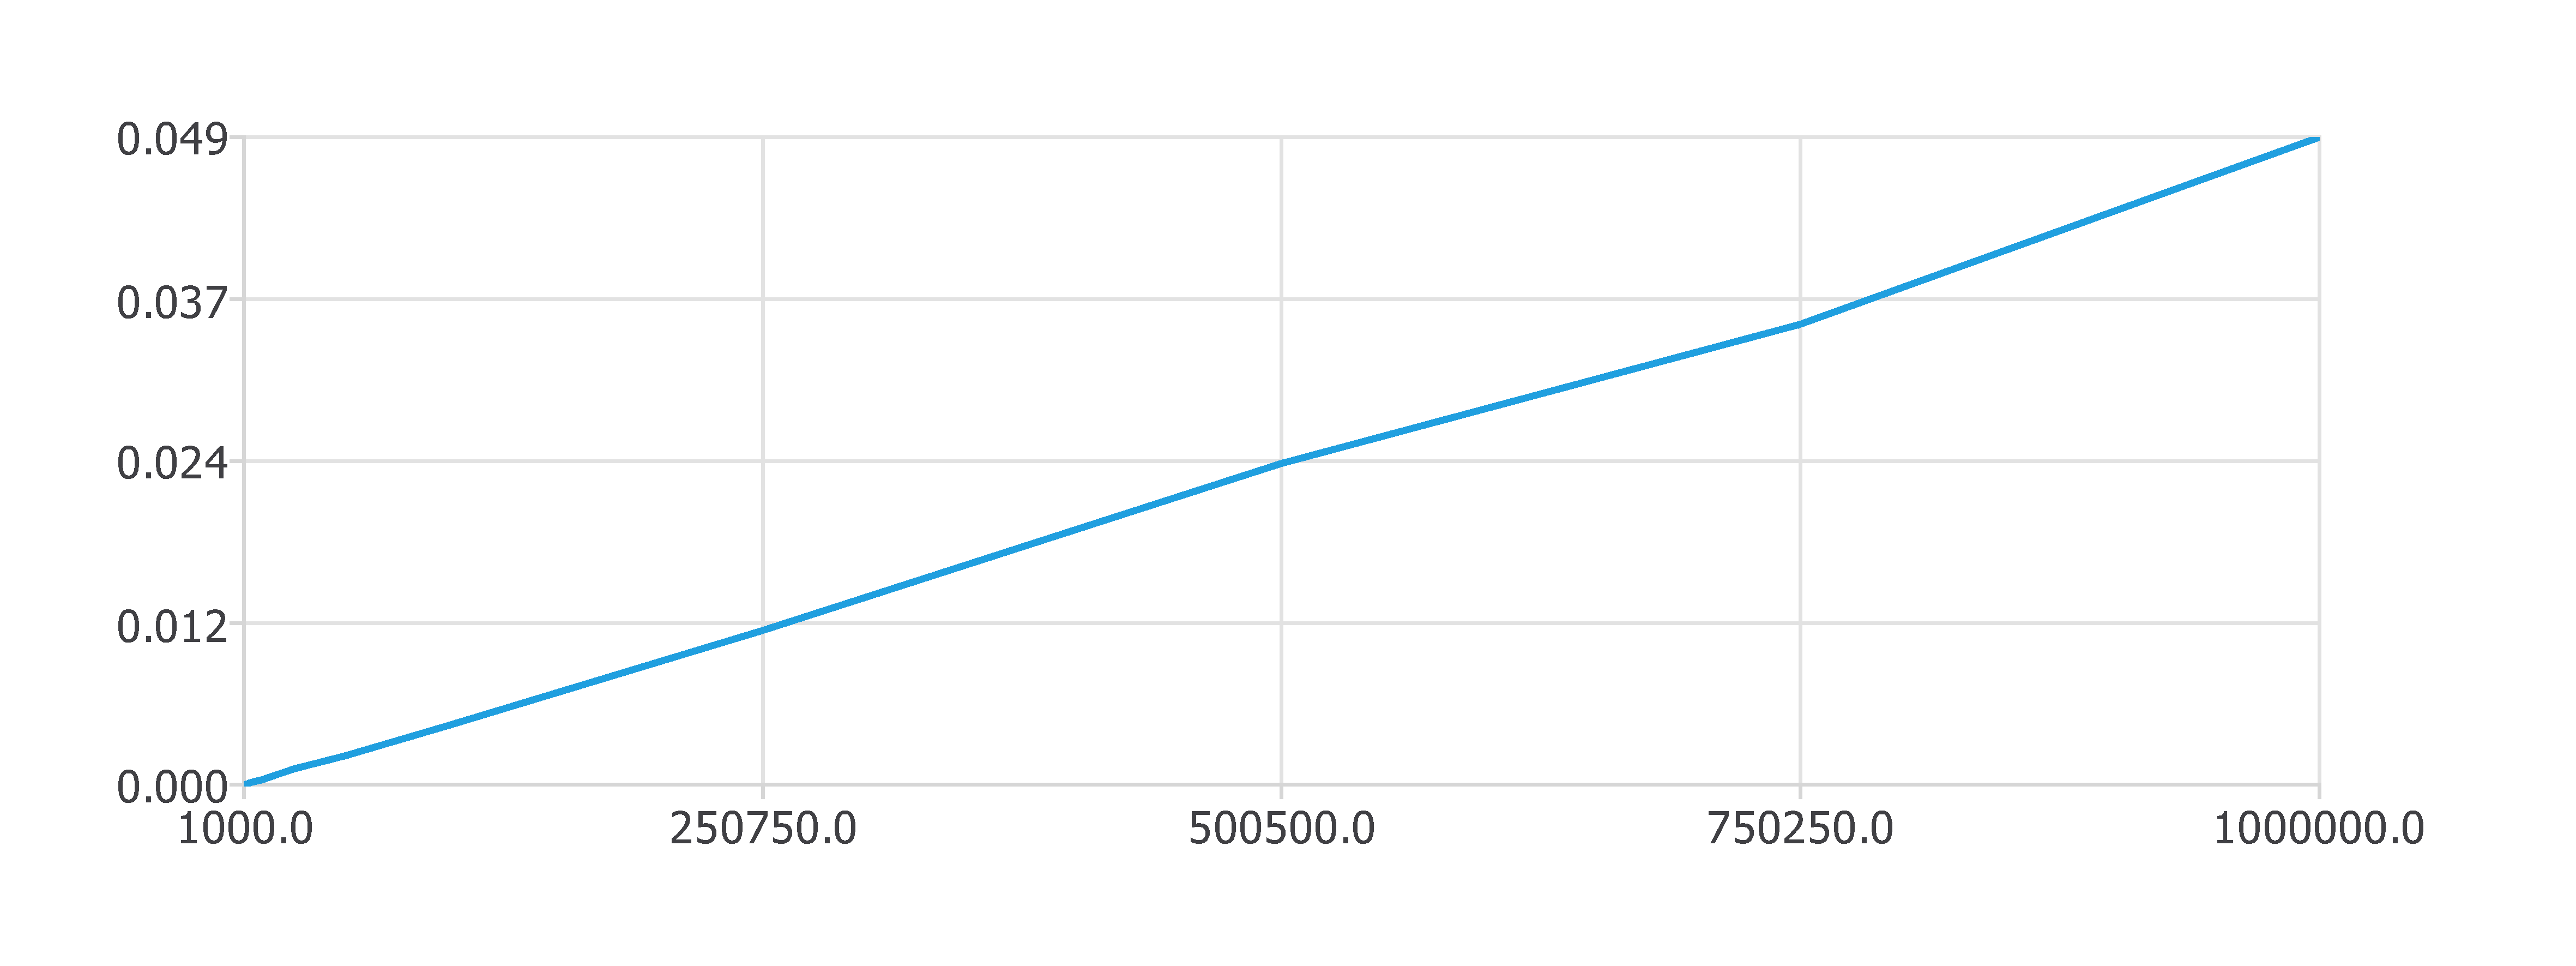
\includegraphics[clip, trim=0cm 0cm 0cm 0cm, width=1\textwidth]{pdf19.pdf}
        \caption{generování}
\end{figure}
\begin{figure}[htbp]
\centering
        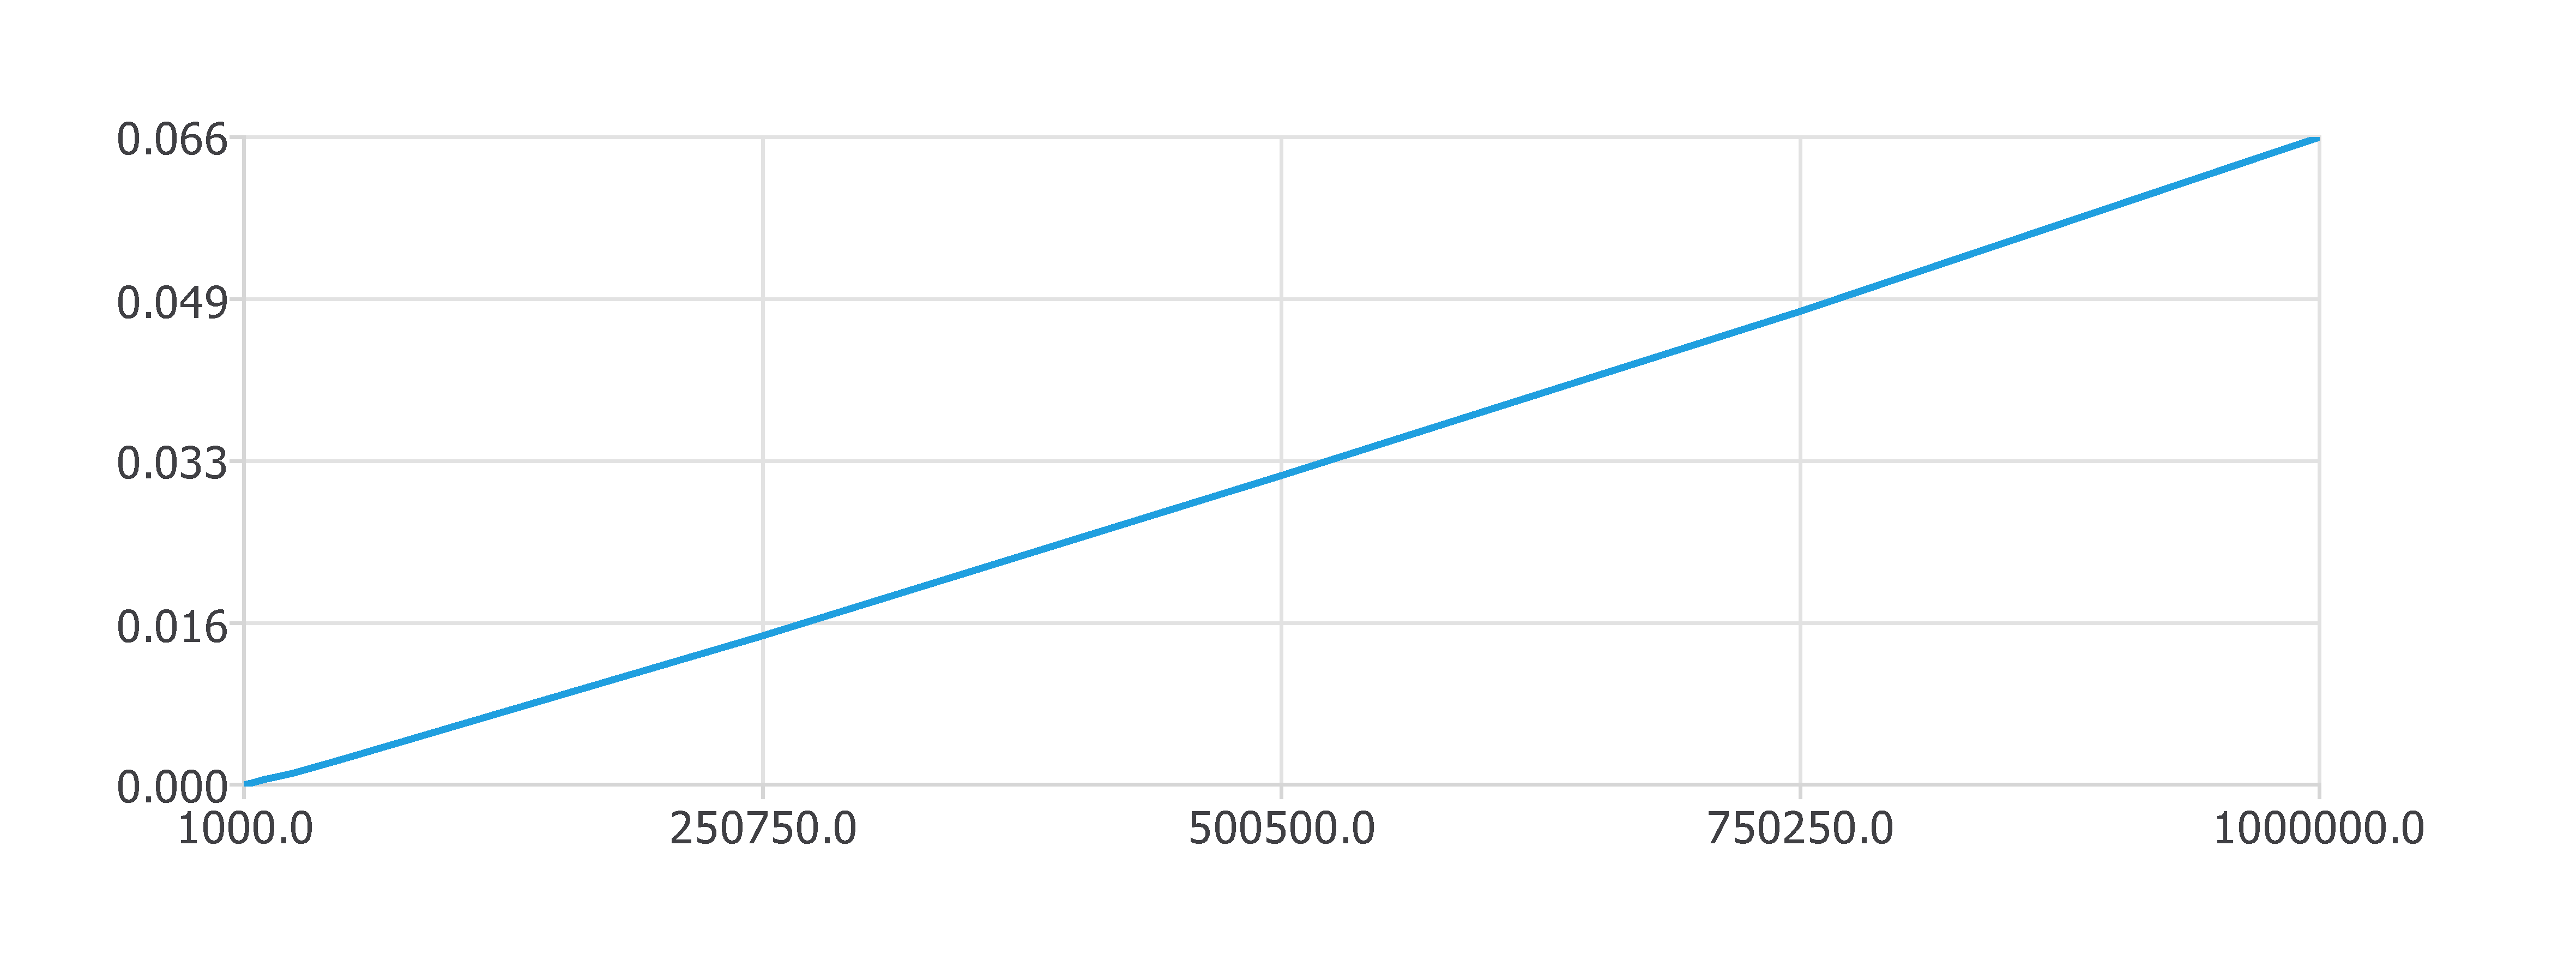
\includegraphics[clip, trim=0cm 0cm 0cm 0cm, width=1\textwidth]{clj.pdf}
        \caption{generování 10x}
\end{figure}
\\
\clearpage
\newpage
\textit{\textbf {Quick Hull}}
\\
\begin{figure}[htbp]
\centering
        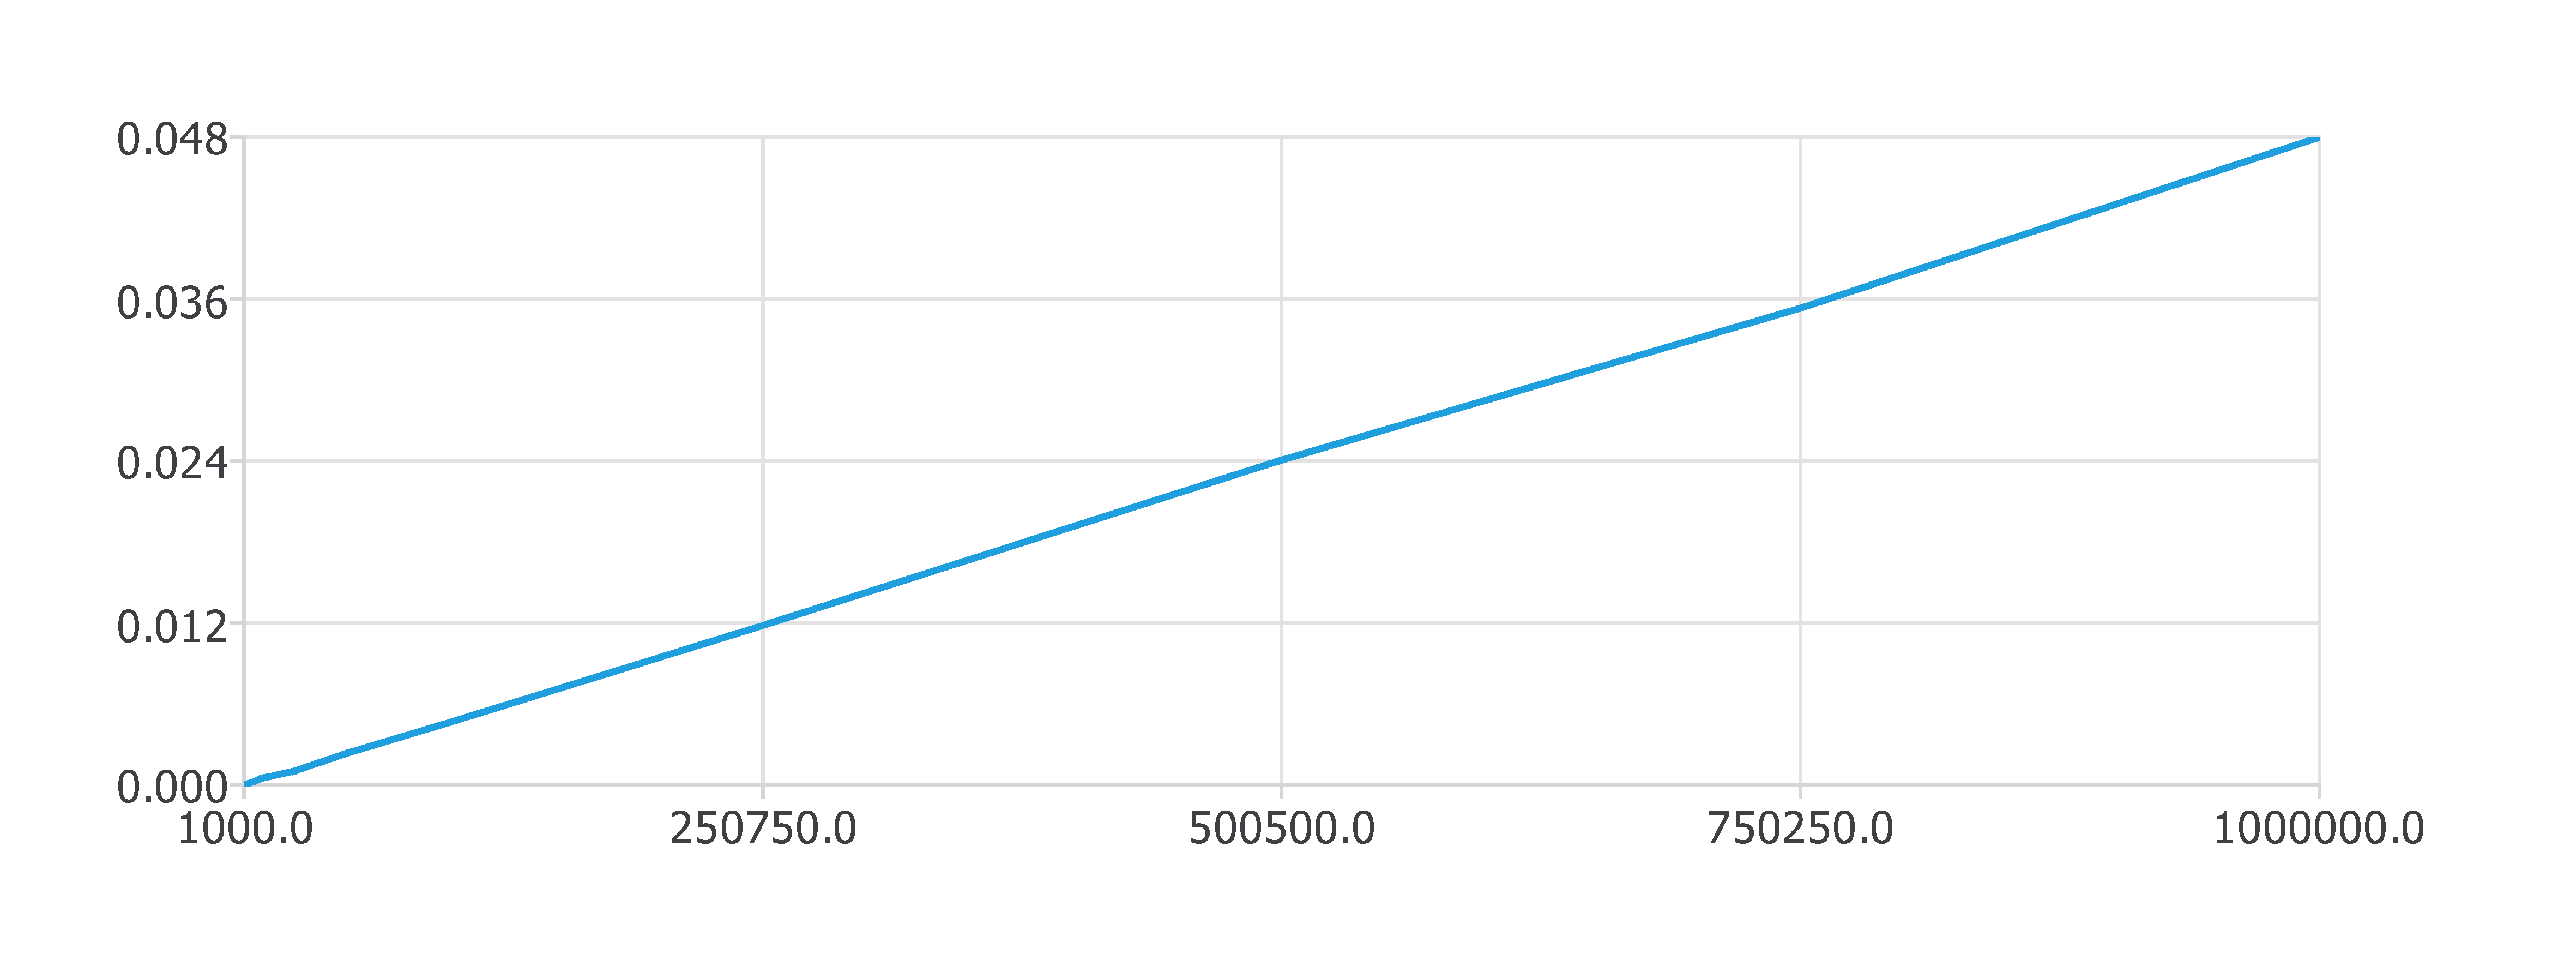
\includegraphics[clip, trim=0cm 0cm 0cm 0cm, width=1\textwidth]{pdf22.pdf}
        \caption{generování}
\end{figure}
\begin{figure}[htbp]
\centering
        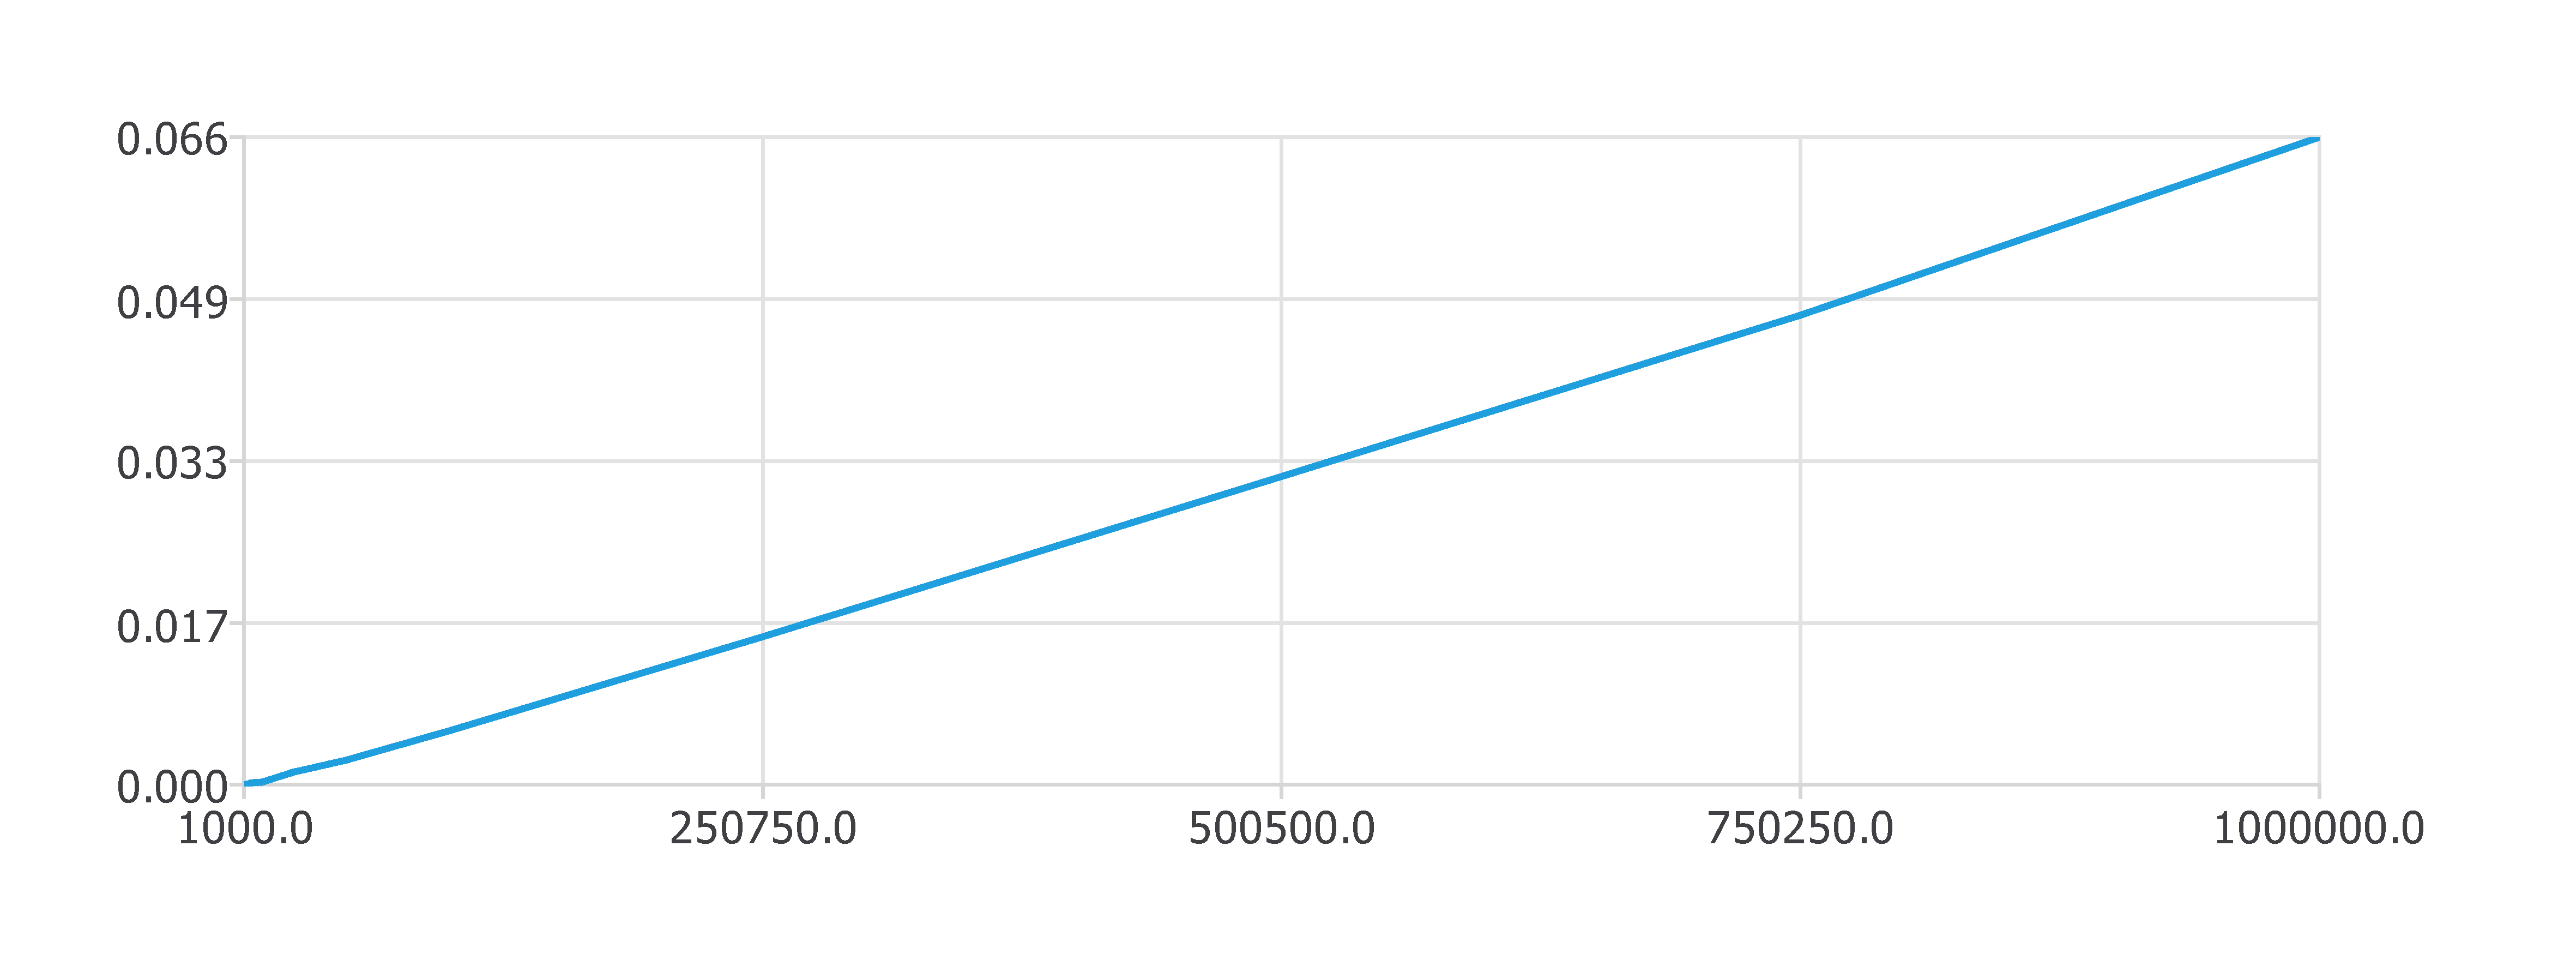
\includegraphics[clip, trim=0cm 0cm 0cm 0cm, width=1\textwidth]{clq.pdf}
        \caption{generování 10x}
\end{figure}
\clearpage
\newpage
\textit{\textbf {Incremental construction}}
\\
\begin{figure}[htbp]
\centering
        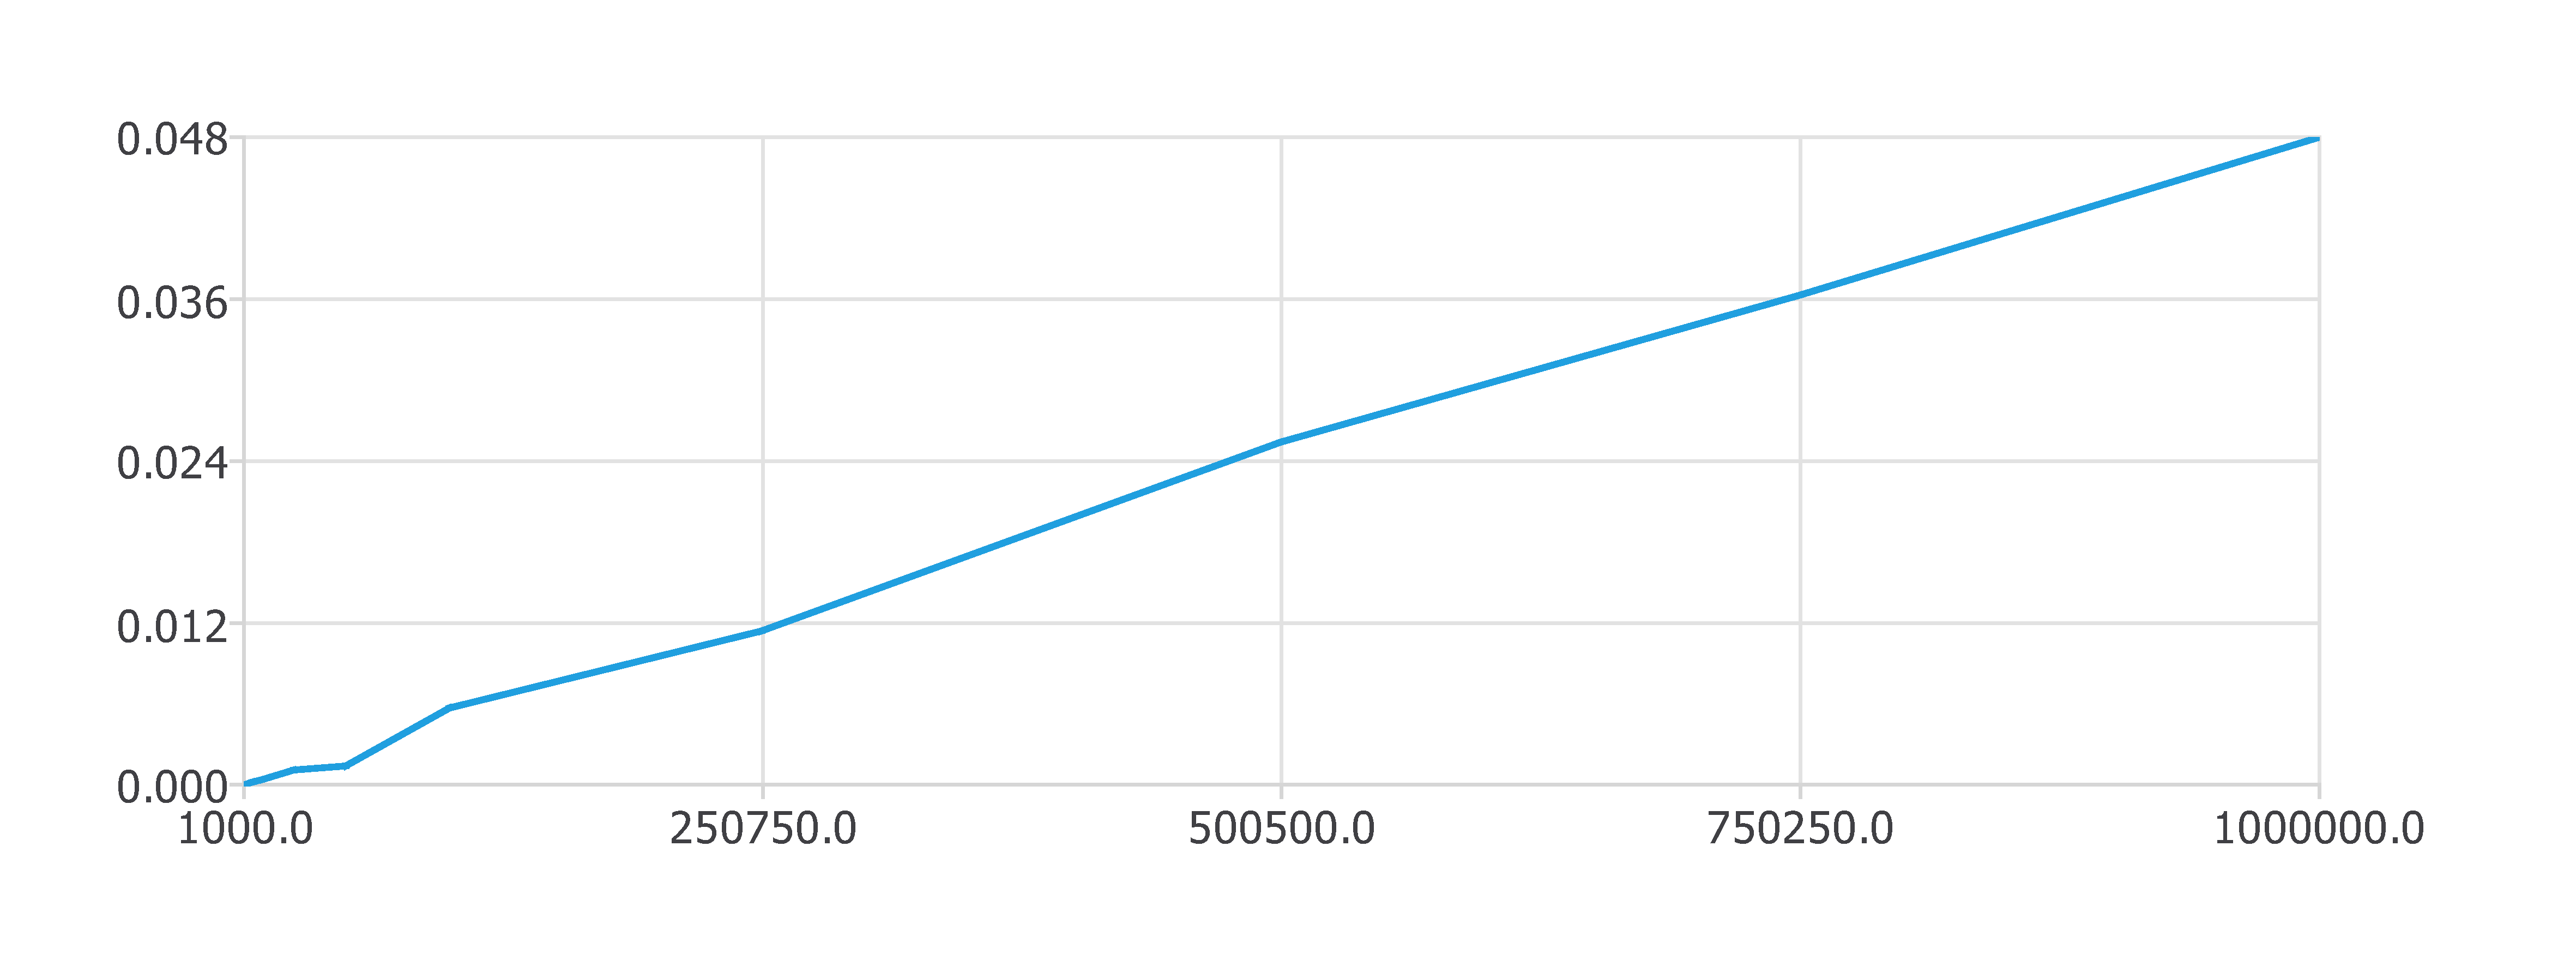
\includegraphics[clip, trim=0cm 0cm 0cm 0cm, width=1\textwidth]{pdf25.pdf}
        \caption{generování}
\end{figure}
\begin{figure}[htbp]
\centering
        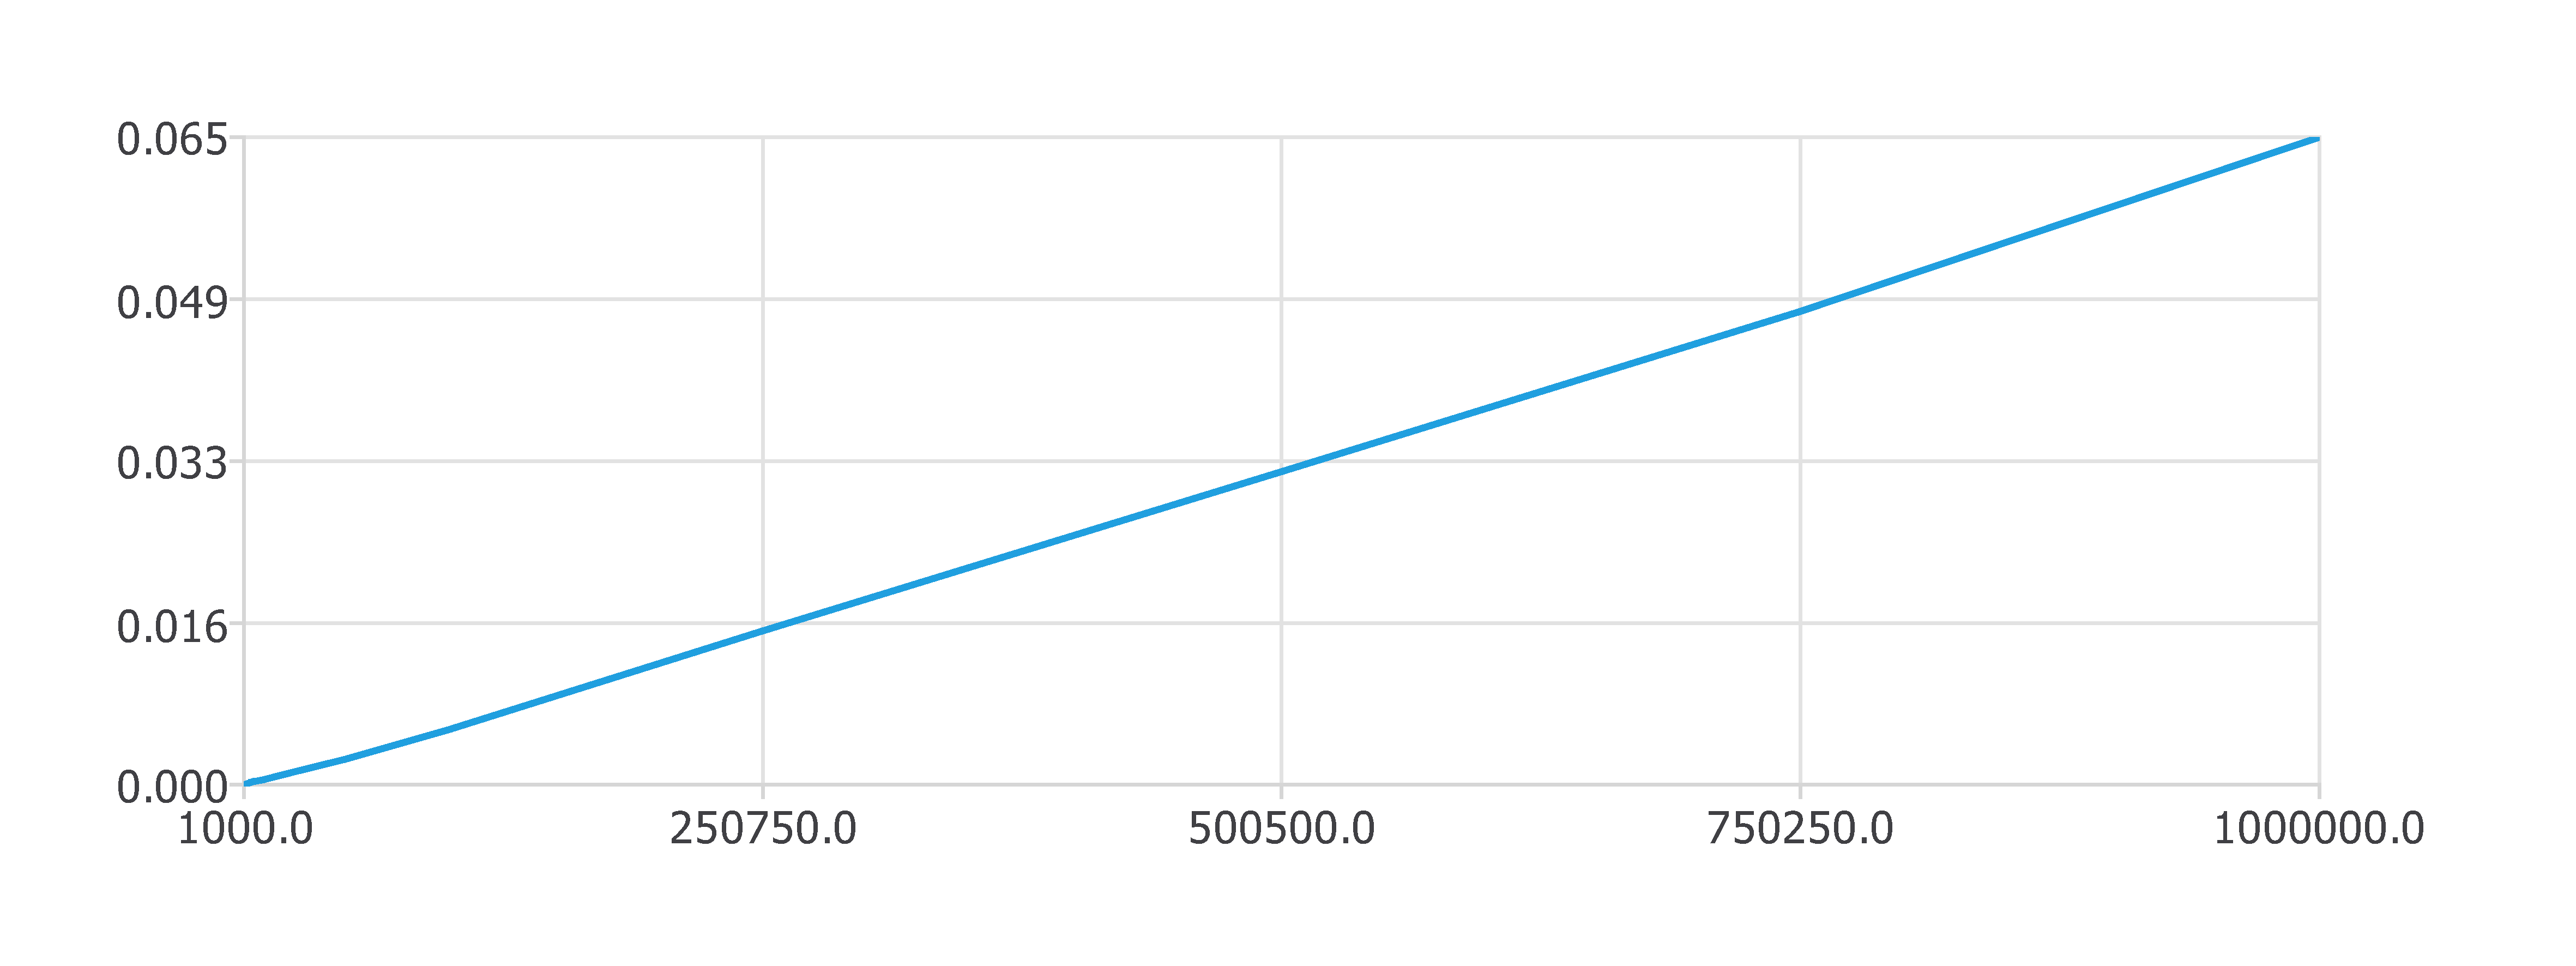
\includegraphics[clip, trim=0cm 0cm 0cm 0cm, width=1\textwidth]{cli.pdf}
        \caption{generování 10x}
\end{figure}
.\\
\bigskip
\clearpage
\section{Závěr}
\indent Autoři splnili většinu bodů zadání a vznikl program, který generuje soubor bodů, jejich rozmíštění a počita rychlost výpočtu algortimu.
V předchozí kapitole jsou zobrazeny grafy, které znázorňují pruběhy výpočtu algoritmů. Test byl proveden několikrát. Jak je vidět z grafů, nejvíce nestabiliní je Jarvis Scan. Dochází k velkému kolisání v počátečných aj dokonce u středních hodnot. O něco lépe je na tom Quick Hull, a však aj u něho dochází ke znáčným výchylům. Obecně dalo by se řici, že Incremental construction je nejvíc stabilní algoritmus ze všech výše uvedených.
\bigskip
Každopádně k výchylům na intervalu hodnot kolem několika tisíc dochází pravidelně a u všech algoritmů. S rostoucím počtem $n$ klesa zároveň výchylka mezi jednotlivými testy. Zároveň s rostoucím počtem $n$ klesa rozdíl mezi jednotilivými metodami. 
\bigskip
Z výsledku lze usoudit, že pro generování menšího objemu dat je lepší využit Incremental construction, případně Quick Hall, naopak pro velký objem dat co převýšuje velikosti desítek tisíc je možné využivát jaký koliv algoritmus.
Bohužel z časových důvodů nebylo možné splnit bonusové úlohy, proto třeba Graham Scan zůstal jen rozdělaný.
	\subsection{Náměty na vylepšení} %+možné či neřešené problémy
	\indent Aplikace, ač funkční a splňující daný účel, má spoustu nedostatků, které by bylo dobré v budoucnu odstranit. Autoři zde uvádí pár těch nejzjevnějších. \\
	\bigskip
	V algoritmu Incremental pro malé hodnoty (cca 10 bodů) dochází k tomu, že občas některý bod není zahrnut do vzníku nové obálky. Bohužel chybu nešlo přimo detekovát, protože má nahodilý charakter.\\
	\bigskip \indent \textit{Souřadnicové osy: }
	\\
	 Vykreslovací okno má v Qt, stejně jako ve většině podobných nástrojů, počátek souřadnic v levém horním rohu, kladnou osu x vpravo a kladnou osu y směrem dolů. Tento model se však neshoduje ani s geodetickými souřadnicemi používanými na našem území (kladná y doleva, kladná x dolů), ani s klasickým označením os (kladná x doprava, kladná y nahoru). Proto se body v současné verzi zobrazují jinak, než by možná uživatel očekával. Vhodným řešením by byla opět transformace. \\
	\bigskip 
\bibliography{u1}
\bibliographystyle{plain}
\addcontentsline{toc}{section}{References}
\pagestyle{empty}

%\end{homeworkSection}
\clearpage

%-----------------------------------------------------------------------------
\end{document}